\chapter{Resultados Obtidos}
Este capítulo demonstra os artefatos produzidos para o \textit{software}, incluindo 
as informações associadas desde a análise até os testes.

\section{Levantamento de Requisitos}

O levantamento de requisitos foi essencial para compreender as necessidades do projeto e orientar o 
desenvolvimento das funcionalidades do aplicativo. Segundo 
\citeonline{sommerville2011}, os requisitos de um sistema são as descrições do que o sistema deve 
fazer, os serviços que ele irá oferecer e suas restrições de funcionamento. Neste projeto, a 
definição dos requisitos prioritários para o MVP\footnote{MVP é a sigla para 
\textit{Minimum Viable Product} (Produto Mínimo Viável), um conceito que se refere à 
versão mais simples de um produto 
que ainda entrega valor ao usuário e permite validações com o mínimo de esforço e 
custo.} e das suas limitações foi orientada por reuniões 
com o coordenador do projeto Fauna Marinha RS, especialmente com base na experiência prática dos 
profissionais do CECLIMAR, que indicaram as funcionalidades mais relevantes para o sistema.

\subsection{Requisitos Funcionais}

Nesta seção, serão expostos os requisitos funcionais do sistema, que segundo 
\citeonline{guedesuml2} correspondem ao que o cliente quer que o sistema realize,
ou seja, as funcionalidades do software. Esses requisitos estão organizados em tabelas
distintas, apresentadas a seguir. A Tabela~\ref{tab:req-funcionais} sintetiza os 63 requisitos funcionais
da versão 2.3.6 do aplicativo, que é a versão mais atualizada até o momento da entrega deste relatório.
Durante o desenvolvimento, os requisitos foram revisados e atualizados conforme necessário,
com base em feedbacks e testes realizados.

\begin{longtable}{@{}p{1.5cm}p{13cm}@{}}
    \caption{Requisitos funcionais do sistema}\label{tab:req-funcionais}\\
        \toprule
        \textbf{Código} & \textbf{Descrição} \\ \hline
        \midrule
        \endfirsthead
        
        \toprule
        \textbf{Código} & \textbf{Descrição} \\ \hline
        \midrule
        \endhead
        
        \midrule
        \multicolumn{2}{r@{}}{(Continua na próxima página)} \\
        \endfoot
        
        \bottomrule
        \endlastfoot
    % usuario
    % registro
    RF01 & O sistema deve permitir o registro de novos usuários com e-mail e senha. \\ \hline
    RF02 & O sistema deve permitir o registro de novos usuários com conta Google integrada ao Firebase Authentication. \\ \hline
    RF03 & O sistema deve diferenciar dois tipos de usuários: cientista cidadão (user) e pesquisador (admin). \\ \hline
    RF04 & O sistema deve permitir que um pesquisador cadastre outro pesquisador, com geração automática de senha segura (8 dígitos alfanuméricos e caracteres especiais). \\ \hline
    RF05 & O sistema deve permitir que um pesquisador conceda a outro usuário que já possui conta a role de pesquisador. \\ \hline

    % login
    RF06 & O sistema deve permitir o login via Firebase Authentication com e-mail e senha. \\ \hline
    RF07 & O sistema deve permitir o login via conta Google integrada ao Firebase Authentication. \\ \hline
    RF08 & O sistema deve unificar dados quando uma conta possui ambos os métodos de login. \\ \hline
    RF09 & O sistema deve permitir redefinição de senha através do fluxo do Firebase Authentication (envio de e-mail de redefinição). \\ \hline
    RF10 & O sistema deve permitir a recuperação da senha. \\ \hline
    RF11 & O sistema deve permitir que o usuário faça logoff. \\ \hline

    % exclusao de conta
    RF12 & O sistema deve permitir a exclusão da conta do usuário, independente do método de cadastro. \\ \hline
    RF13 & O sistema deve manter os registros realizados pelo usuário mesmo após a exclusão da conta, 
    para preservação de dados científicos. \\ \hline

    % editar perfil
    RF14 & O sistema deve permitir atualização do perfil de usuário cadastrado com e-mail e senha (nome, foto, e-mail). \\ \hline
    
    % tela de meu perfil
    RF15 & O sistema deve permitir ao usuário visualizar e gerenciar seu perfil. \\ \hline
    RF16 & O sistema deve possuir um conjunto de conquistas para cada usuário. \\ \hline
    RF17 & O sistema deve permitir ao usuário visualizar os últimos registros do seu perfil. \\ \hline
    RF18 & O sistema deve permitir ao usuário visualizar a quantidade total de registros realizadas por ele. \\ \hline

    % envio de registros
    RF19 & O sistema deve permitir envio de registros "simples". \\ \hline
    RF20 & O sistema deve permitir envio de registros "técnicos" com dados mais específicos. \\ \hline
    RF21 & O sistema deve permitir envio de até 2 imagens por registro, sendo uma obrigatória. \\ \hline
    RF22 & O sistema deve permitir envio de registros utilizando GPS do dispositivo em tempo real para obter as coordenadas geográficas. \\ \hline
    RF23 & O sistema deve validar os formulários de envio de registros com restrições específicas (ex.: limite de caracteres). \\ \hline
    RF24 & O sistema deve permitir que o usuário envie uma imagem a partir da galeria do celular. \\ \hline
    RF25 & O sistema deve permitir que o usuário envie uma imagem a partir da camera do celular. \\ \hline
    RF26 & O sistema deve permitir consultar dados de geolocalização a partir das. \\ \hline
    RF27 & O sistema deve permitir envio de registros utilizando a opção número da guarita para basear as coordenadas geográficas. \\ \hline
    RF28 & O sistema deve permitir envio de registros utilizando coordenadas da cidade para definir a localização. \\ \hline
    RF29 & O sistema deve permitir envio de registros utilizando ponto de referência como campo aberto. \\ \hline
    RF30 & O sistema deve facilitar a ativação da geolocalização do dispositivo pelo usuário. \\ \hline
    RF31 & O sistema deve permitir visualizar a imagem de um registro em tela cheia. \\ \hline
    RF32 & O sistema deve exibir o nome da cidade automaticamente com base na localização do registro. \\ \hline
    RF33 & O sistema deve permitir o armazenamento de registros quando enviados offline. \\ \hline

    %sobre 
    RF34 & O sistema deve apresentar uma tela com informações sobre o projeto e os desenvolvedores. \\ \hline

    % meus registros
    RF35 & O sistema deve permitir que o usuário visualize todos registros que ele enviou. \\ \hline
    RF36 & O sistema deve permitir que o usuário filtre os registros enviados e já validados. \\ \hline
    RF37 & O sistema deve permitir que o usuário receba o retorno do profissional para cada registro. \\ \hline
    RF38 & O sistema deve permitir que um pesquisador delete um registro enviado por qualquer usuário. \\ \hline
    RF39 & O sistema deve permitir a visualização detalhada de um registro selecionado. \\ \hline
    
    % interface
    RF40 & O sistema deve apresentar uma barra de navegação fixa com as opções: início, registros, 
    novo registro, perfil e sobre. \\ \hline
    RF41 & O sistema deve apresentar um menu inicial com todas as funcionalidades disponíveis. \\ \hline
    RF42 & O sistema deve assegurar que apenas usuários pesquisadores tenham acesso a algumas funcionalidades. \\ \hline
    RF43 & O sistema deve possuir uma seção para apresentar os principais animais da fauna local. \\ \hline
    RF44 & O sistema deve possuir uma tela de carregamento inicial. \\ \hline

    % painel de registros
    RF45 & O sistema deve permitir que o usuário visualize os registros enviados por outros usuários. \\ \hline
    RF46 & O sistema deve disponibilizar um painel de registros com estatísticas, mapas e filtros detalhados para acompanhamento. \\ \hline
    RF47 & O sistema deve permitir que os usuários comuns exportem um arquivo CSV com dados sensíveis ocultos. \\ \hline
    RF48 & O sistema deve permitir que os pesquisadores exportem um arquivo CSV com os dados gerais dos registros. \\ \hline
    RF49 & O sistema deve permitir que sejam vistos todos os registros enviados ainda não avaliados. \\ \hline
    RF50 & O sistema deve permitir que sejam vistos todos os registros já avaliados. \\ \hline
    RF51 & O sistema deve apresentar um mapa interativo com pontos de registros. \\ \hline
    RF52 & O sistema deve apresentar os animais que possuem mais registros documentados. \\ \hline
    RF53 & O sistema deve incrementar o número de encontros com cada espécie após uma avaliação de pesquisador. \\ \hline
    RF54 & O sistema deve possuir um contador por classe para os mamíferos, as aves e os répteis. \\ \hline
    RF55 & O sistema deve permitir a busca de registros por espécie. \\ \hline
    RF56 & O sistema deve permitir a busca de número de registros dentro de uma faixa de tempo. \\ \hline

    % avaliacao de registros
    RF57 & O sistema deve permitir que pesquisadores avaliem de todos os registros enviados. \\ \hline
    RF58 & O sistema deve permitir a inserção de novos animais no banco de dados. \\ \hline
    RF59 & O sistema deve permitir que o pesquisador adicione comentários aos registros enviados. \\ \hline
    RF60 & O sistema deve permitir que os dados enviados por um usuário sejam editáveis para um pesquisador realizar
    a avaliação. \\ \hline
    RF61 & O sistema deve permitir ao pesquisador atualizar a localização ao avaliar um registro. \\ \hline

    % fauna local
    RF62 & O sistema deve redirecionar para o site do projeto Fauna Marinha RS para dados da fauna local. \\ \hline
    RF63 & O sistema deve redirecionar para as redes sociais do projeto Fauna Marinha RS. \\ \hline
\end{longtable}
\legend{Fonte: Autor}

\subsection{Requisitos Não Funcionais}

Segundo \citeonline{pressman2011engenharia}, os requisitos não funcionais podem ser descritos 
como uma característica de qualidade, desempenho, segurança ou restrição geral de um sistema. 
Na Tabela~\ref{tab:req-nao-funcionais}, temos o detalhamento desses requisitos, com a finalidade 
de sintetizar as propriedades essenciais que asseguram o bom funcionamento da aplicação. 
Tais requisitos são fundamentais 
para garantir aspectos como usabilidade, confiabilidade, portabilidade e eficiência, além de assegurar 
conformidade com as tecnologias e práticas adotadas no desenvolvimento do sistema.

\begin{longtable}{@{}p{1.5cm}p{13cm}@{}}
    \caption{Requisitos não funcionais do sistema}\label{tab:req-nao-funcionais}\\
    \toprule
    \textbf{Código} & \textbf{Descrição} \\ \hline
    \midrule
    \endfirsthead
    
    \toprule
    \textbf{Código} & \textbf{Descrição} \\ \hline
    \midrule
    \endhead
    
    \midrule
    \multicolumn{2}{r@{}}{(Continua na próxima página)} \\
    \endfoot
    
    \bottomrule
    \endlastfoot
    RNF01 & O sistema deve ser desenvolvido utilizando Flutter e Dart, garantindo compatibilidade 
    multiplataforma. \\ \hline
    RNF02 & O sistema deve utilizar autenticação segura via Firebase, com criptografia adequada para 
    senhas e tokens. \\ \hline
    RNF03 & O sistema deve apresentar alta disponibilidade e ser resiliente a falhas de rede. \\ \hline
    RNF04 & O sistema deve indicar quando alguma funcionalidade não está disponível. \\ \hline
    RNF05 & O sistema deve seguir as melhores práticas de UX, com validação clara de formulários e 
    feedbacks visuais para os usuários. \\ \hline
    RNF06 & O sistema deve garantir a privacidade dos dados do usuário, omitindo dados sensíveis em 
    exportações para cientistas cidadãos. \\ \hline
    RNF07 & O sistema deve apresentar desempenho aceitável mesmo em dispositivos móveis de média 
    capacidade. \\ \hline
    RNF08 & O sistema deve fornecer acessibilidade básica, permitindo navegação simples e intuitiva. \\ \hline
    RNF09 & O sistema deve apresentar feedbacks constantes sobre os status de processamento da aplicação. \\ \hline
    RNF10 & O sistema deve ser inicialmente disponibilizado para Android. \\ \hline
\end{longtable}
\legend{Fonte: Autor}

\section{Prototipação da Interface com o Usuário}
A prototipação foi dividida em quatro etapas principais, com foco na representação 
visual da aplicação e na simulação dos fluxos de navegação dos usuários. A seguir, 
são descritas as fases de prototipação realizadas.

\subsection{Definição da Identidade Visual}

A identidade visual do aplicativo foi construída com base nos elementos gráficos já 
existentes no projeto Fauna Marinha RS (Figura~\ref{fig:identidade-visual-web}). Foram 
utilizadas cores similares e o logotipo oficial do projeto, com o objetivo de manter a 
coerência visual entre as diferentes aplicações e garantir o reconhecimento por parte dos 
usuários já familiarizados com a identidade do projeto.

A paleta de cores foi definida de modo a remeter ao ambiente marinho, utilizando tons de 
azul e uma textura que remete à água. Essa paleta é apresentada na Figura~\ref{fig:paleta-cores}.

\begin{figure}[H]
    \centering
    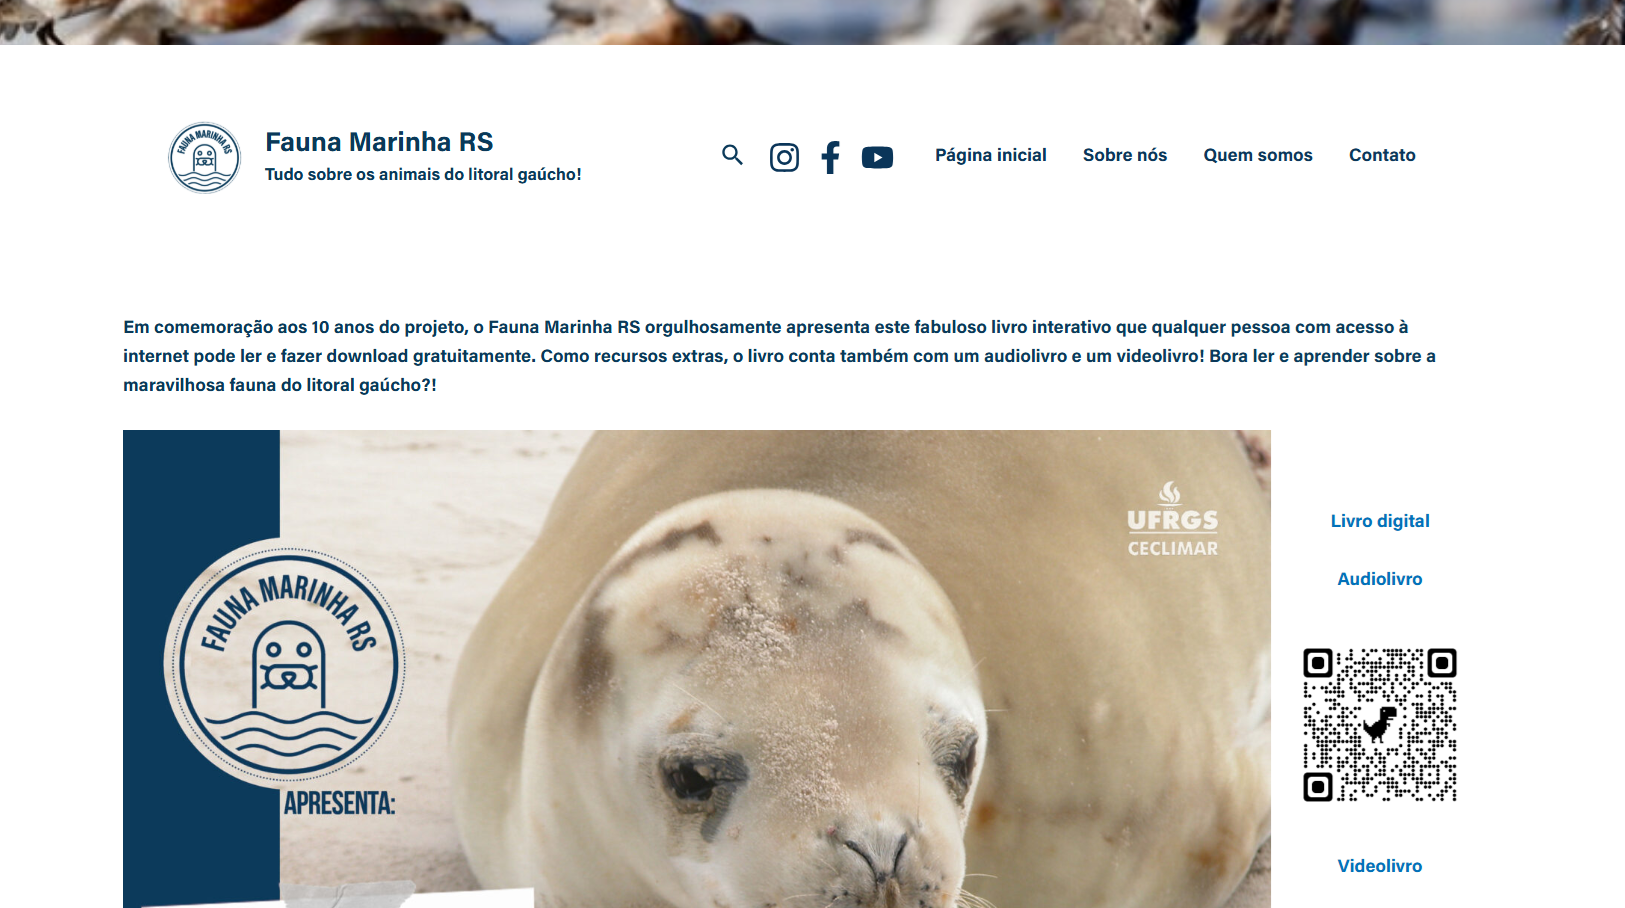
\includegraphics[width=1\textwidth]{imagens/sistemaWebFaunaMar.png}
    \caption{Identidade visual do sistema web do projeto Fauna Marinha RS.}
    \label{fig:identidade-visual-web}
\end{figure}
\legend{Fonte: \cite{faunamarinha2025}}

\begin{figure}[H]
    \centering
    
\includegraphics[height=0.5\textheight]{imagens/identidade-app.png}
    \caption{Identidade visual prototipada.}
    \label{fig:identidade-visual-mobile}
\end{figure}
\legend{Fonte: Autor}

\begin{figure}[H]
    \centering
    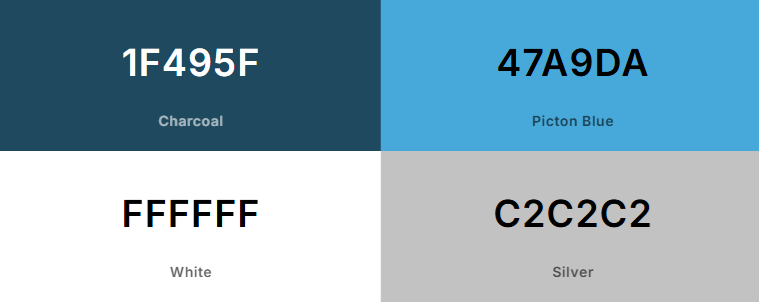
\includegraphics[width=1\textwidth]{imagens/paleta-cores.png}
    \caption{Paleta de cores utilizada.}
    \label{fig:paleta-cores}
\end{figure}
\legend{Fonte: Autor}

\subsection{Criação do Design das Telas}

Com base na identidade visual definida, foram elaborados os layouts das principais telas do 
aplicativo. Essa etapa concentrou-se na organização dos elementos de interface, na 
usabilidade e na experiência do usuário.

Inicialmente, foram criadas as telas de login (Figura~\ref{fig:prototipo-login}) e de 
registro de usuário (Figura~\ref{fig:prototipo-cadastro}).

\begin{figure}[H]
    \centering
    \begin{minipage}[b]{0.48\textwidth}
        \centering
        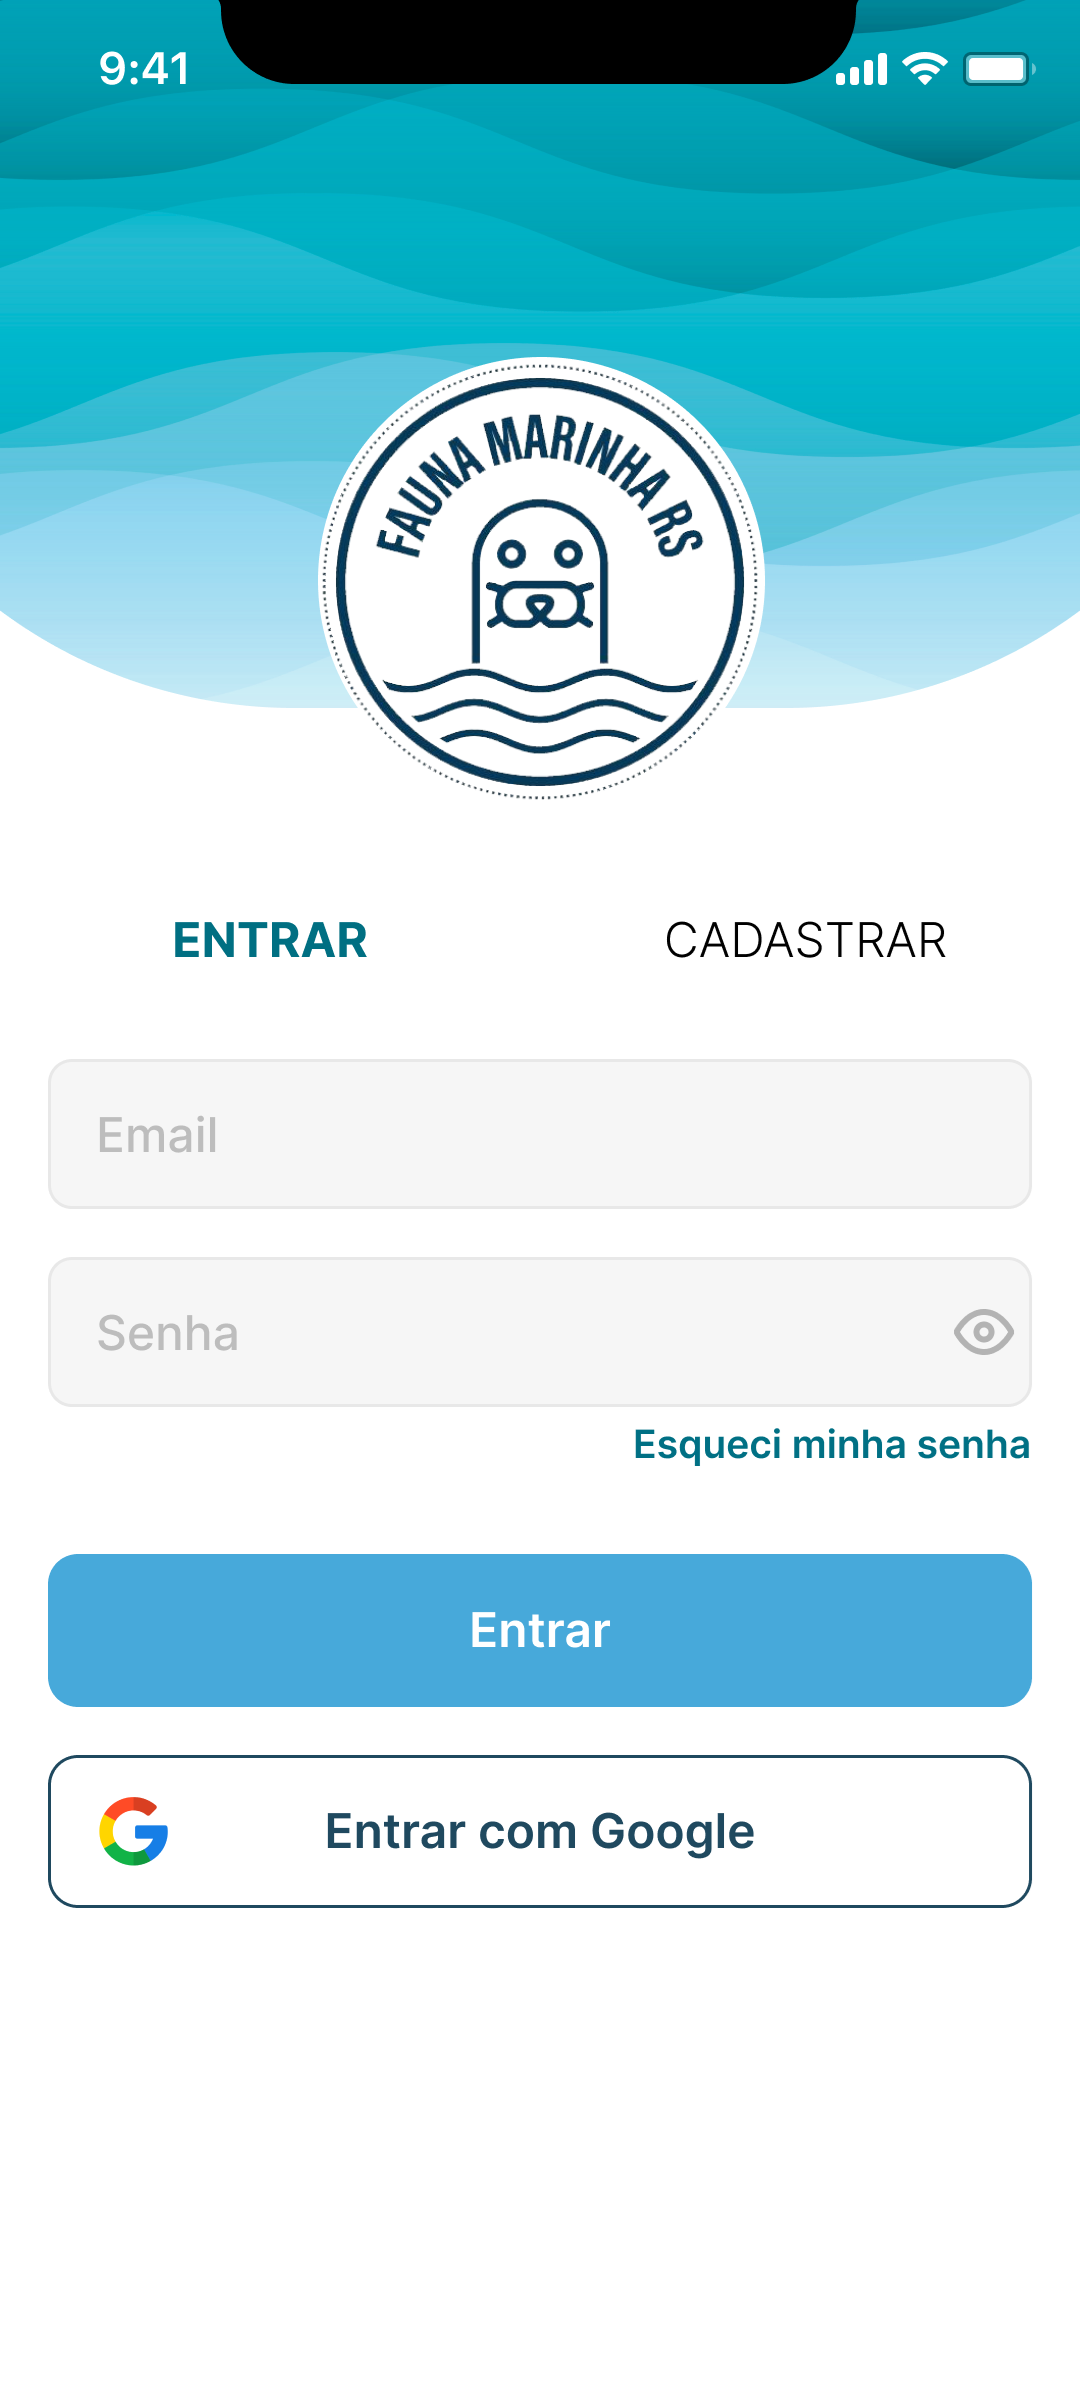
\includegraphics[height=0.6\textheight]{imagens/login-figma.png}
        \caption{Protótipo da tela de login do aplicativo.}
        \label{fig:prototipo-login}
    \end{minipage}
    \hfill
    \begin{minipage}[b]{0.48\textwidth}
        \centering
        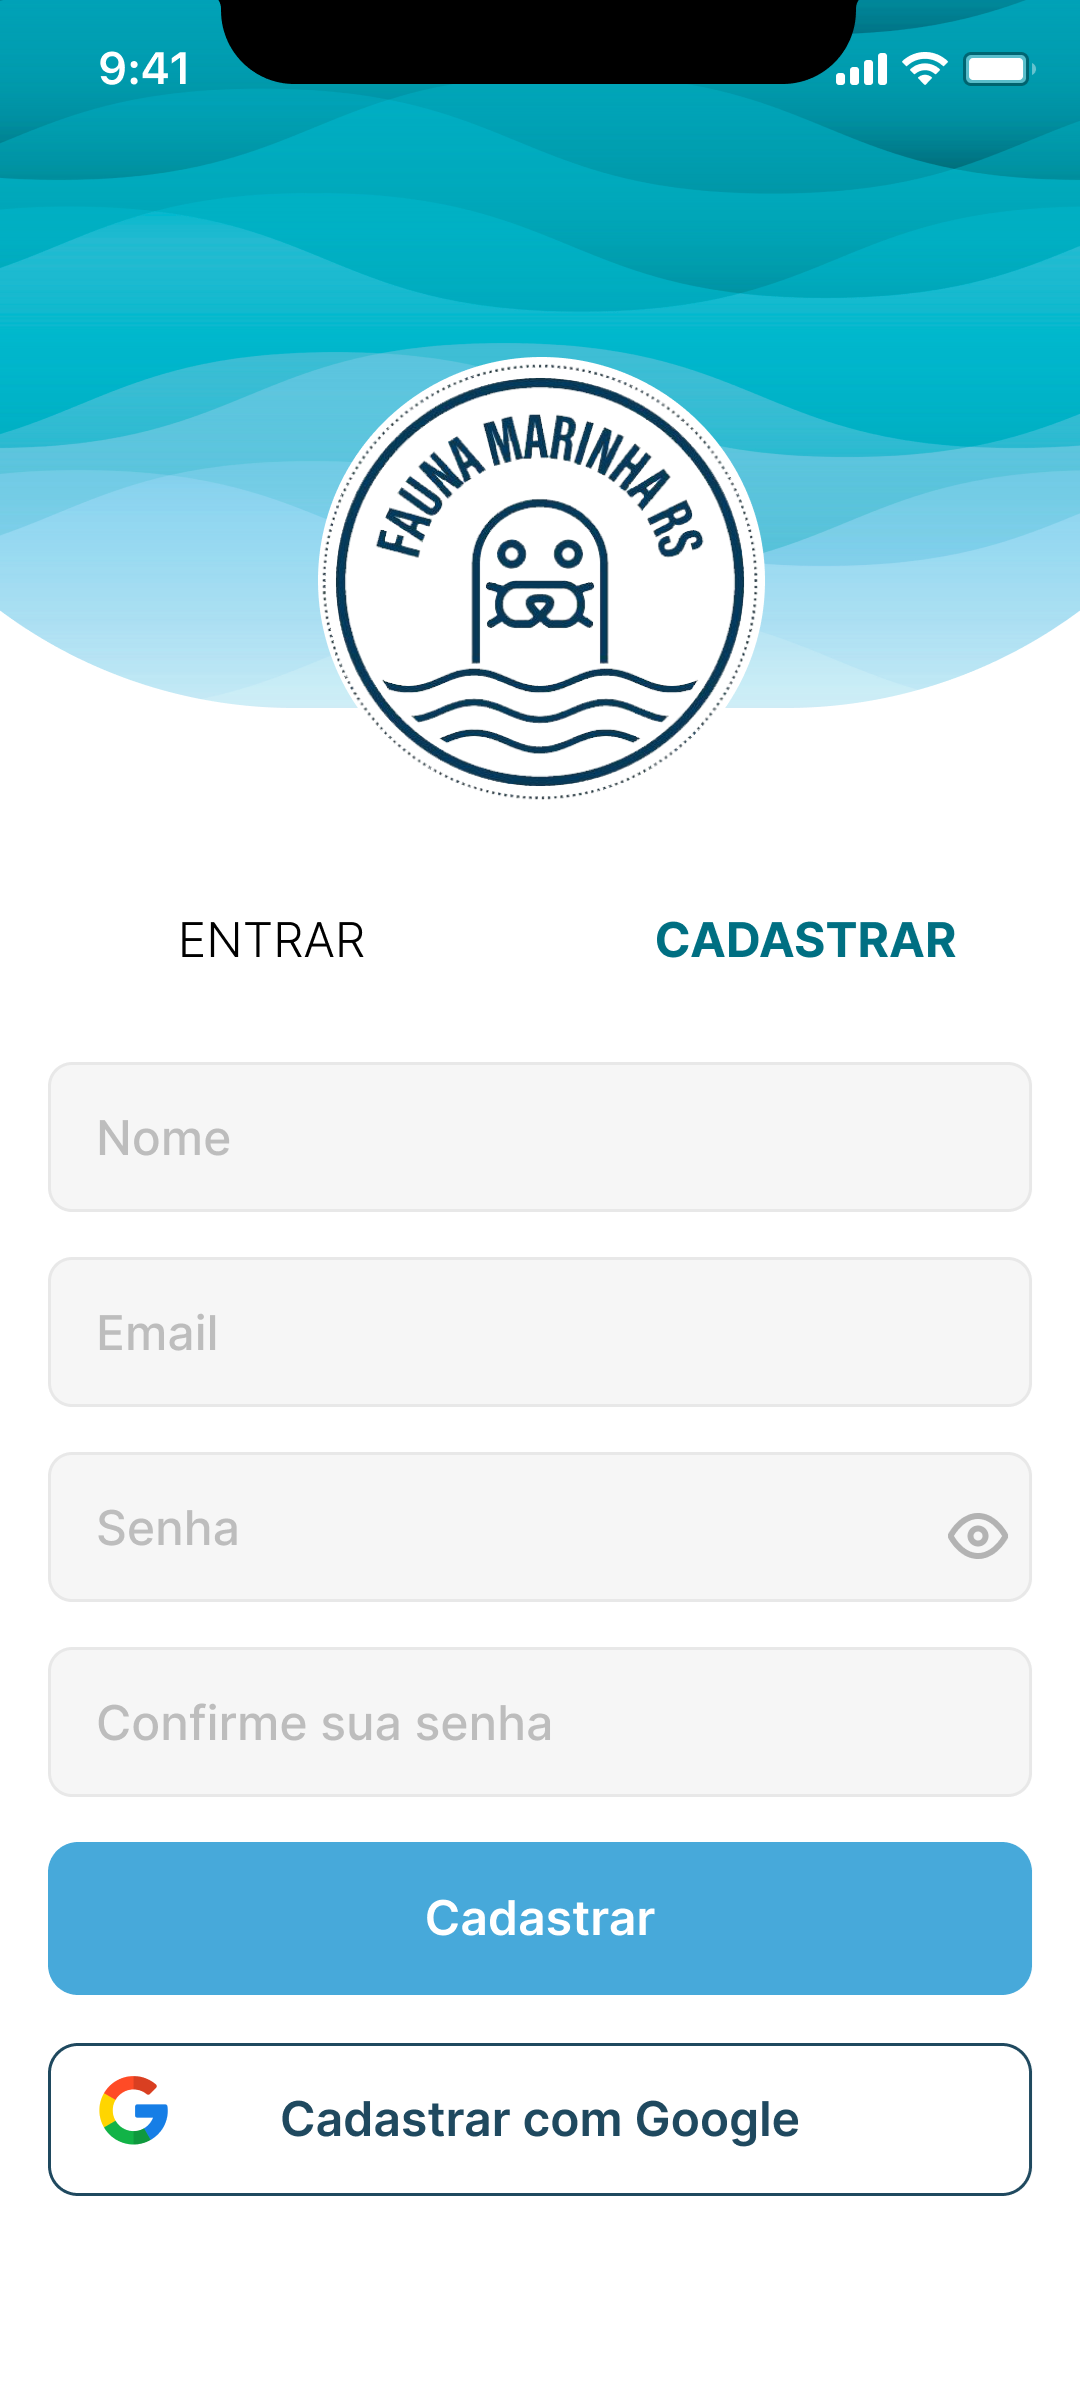
\includegraphics[height=0.6\textheight]{imagens/cadastro-figma.png}
        \caption{Protótipo da tela de cadastro do aplicativo.}
        \label{fig:prototipo-cadastro}
    \end{minipage}
\end{figure}
\legend{Fonte: Autor}

Em seguida, foi criada a tela inicial (Figura~\ref{fig:prototipo-home}), com duas 
variações: uma para usuários comuns e outra para pesquisadores. O layout foi pensado 
para facilitar o acesso às funcionalidades, com botões de acesso rápido e 
barra de navegação fixa na parte inferior da tela. A versão para pesquisadores apresenta os mesmos botões,
com a adição das funcionalidades exclusivas, avaliação de registros e acesso ao painel geral.

\begin{figure}[H]
    \centering
    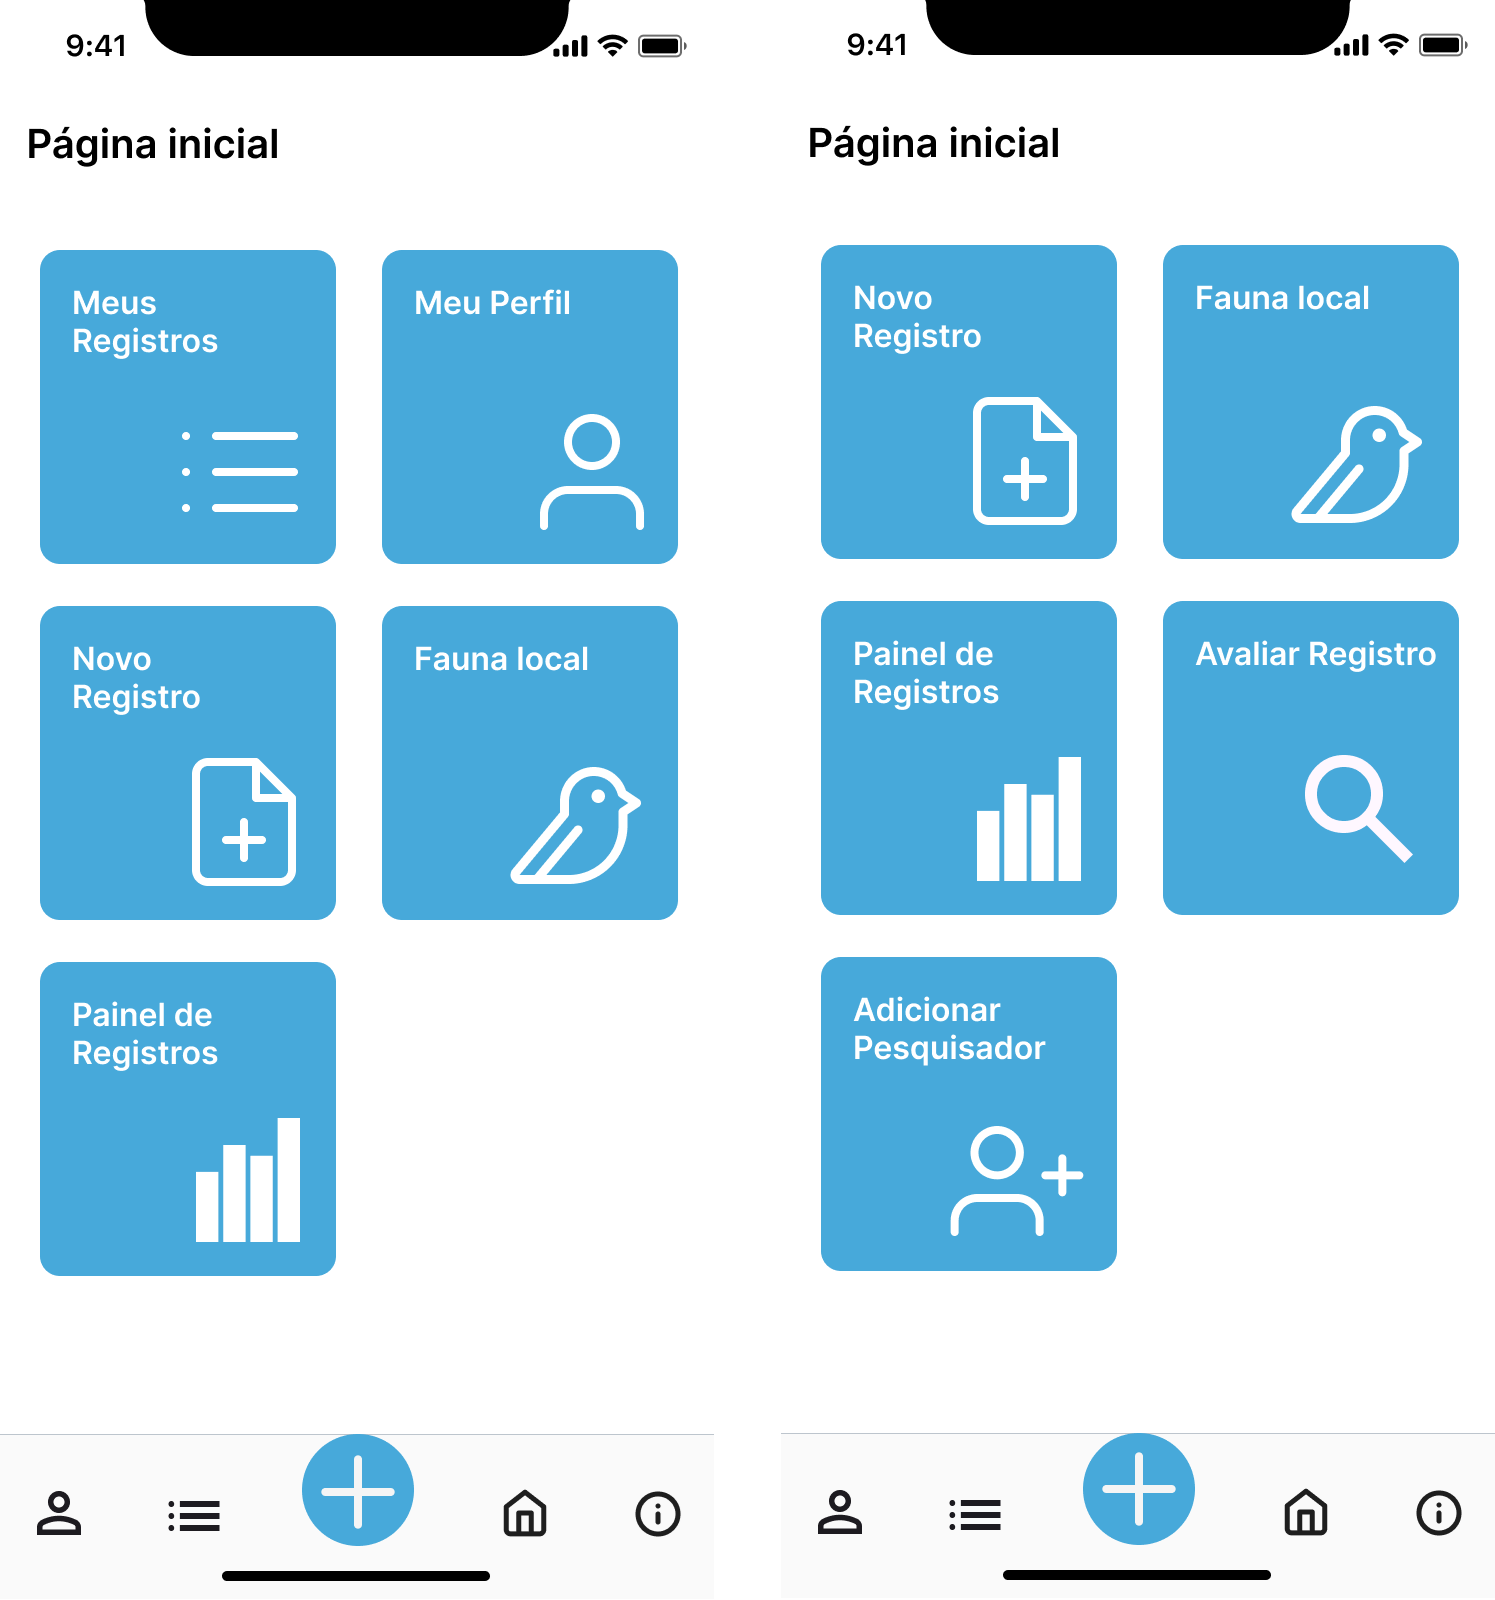
\includegraphics[height=0.6\textheight]{imagens/menu-pesquisador-figma.png}
    \caption{Protótipo da tela inicial: usuário comum (esquerda) e pesquisador (direita).}
    \label{fig:prototipo-home}
\end{figure}
\legend{Fonte: Autor}

A tela "Meus Registros" (Figura~\ref{fig:prototipo-meus-registros}) permite ao usuário 
visualizar todos os registros já enviados, com filtros por status (enviado e validado). 
Também foi projetado um estado com \textit{bottomsheet} acionado a partir do botão de adicionar 
registro ("+") na barra de navegação. Esse botão está disponível em qualquer tela, permitindo 
adicionar registros rapidamente.

\begin{figure}[H]
    \centering
    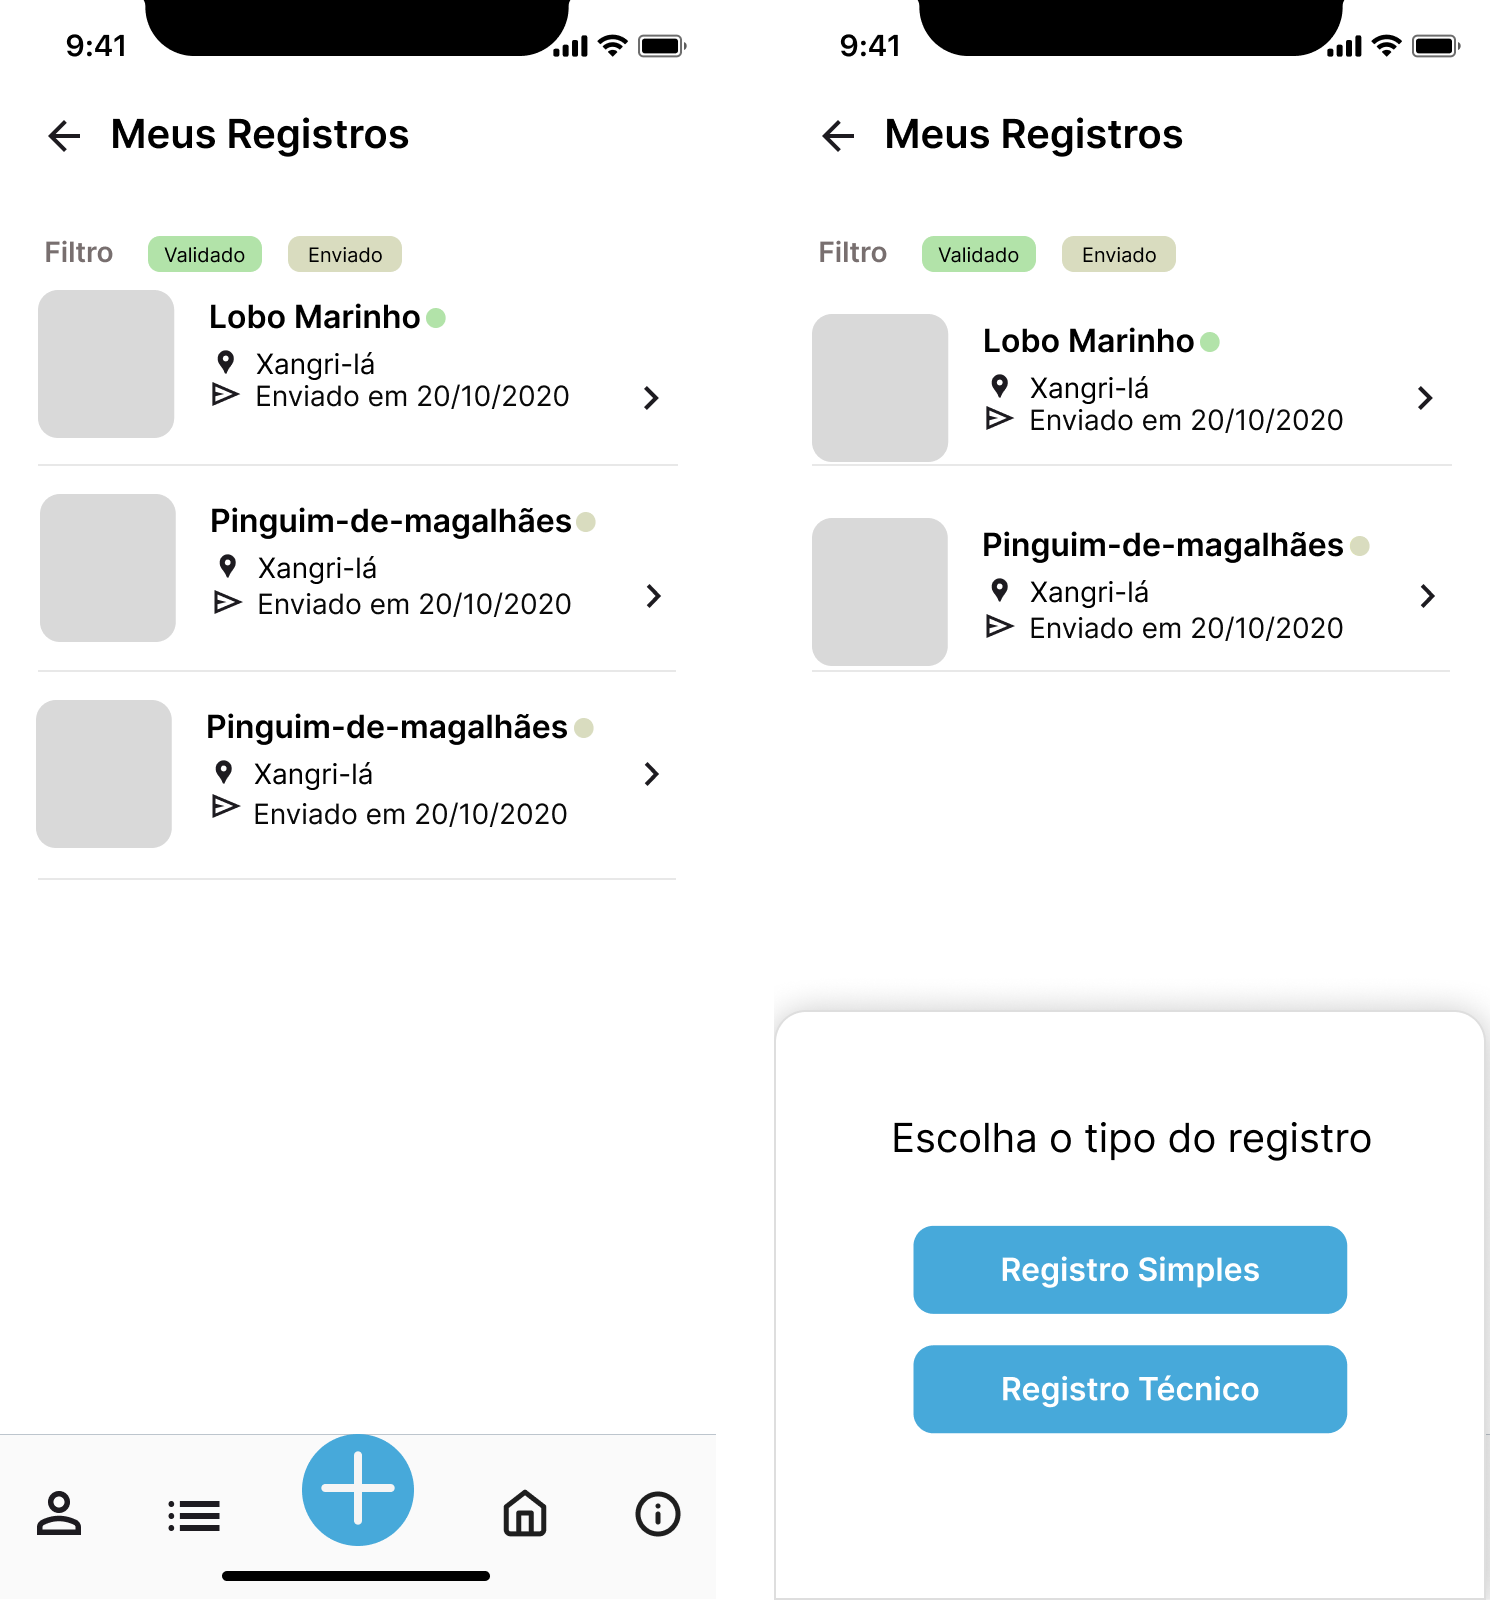
\includegraphics[height=0.6\textheight]{imagens/meus-registros-figma.png}
    \caption{Tela de "Meus Registros" com estado ativo de adição de registro (direita).}
    \label{fig:prototipo-meus-registros}
\end{figure}
\legend{Fonte: Autor}

Dois tipos de formulários de registro foram projetados: um simples
 (Figura~\ref{fig:prototipo-registro-simples}), voltado a usuários leigos e envios rápidos, e 
 outro técnico (Figura~\ref{fig:prototipo-registro-tecnico}), com campos adicionais 
 para coleta de dados mais detalhados. Ambos possuem validações, campos obrigatórios e 
 opcionais, e suporte ao envio de imagens com orientações apresentadas em \textit{bottomsheet}.

Os campos específicos de classe, ordem, família e gênero foram projetados para serem um dropdown,
que apresentará as opções disponíveis para o usuário selecionar.

\begin{figure}[H]
    \centering
    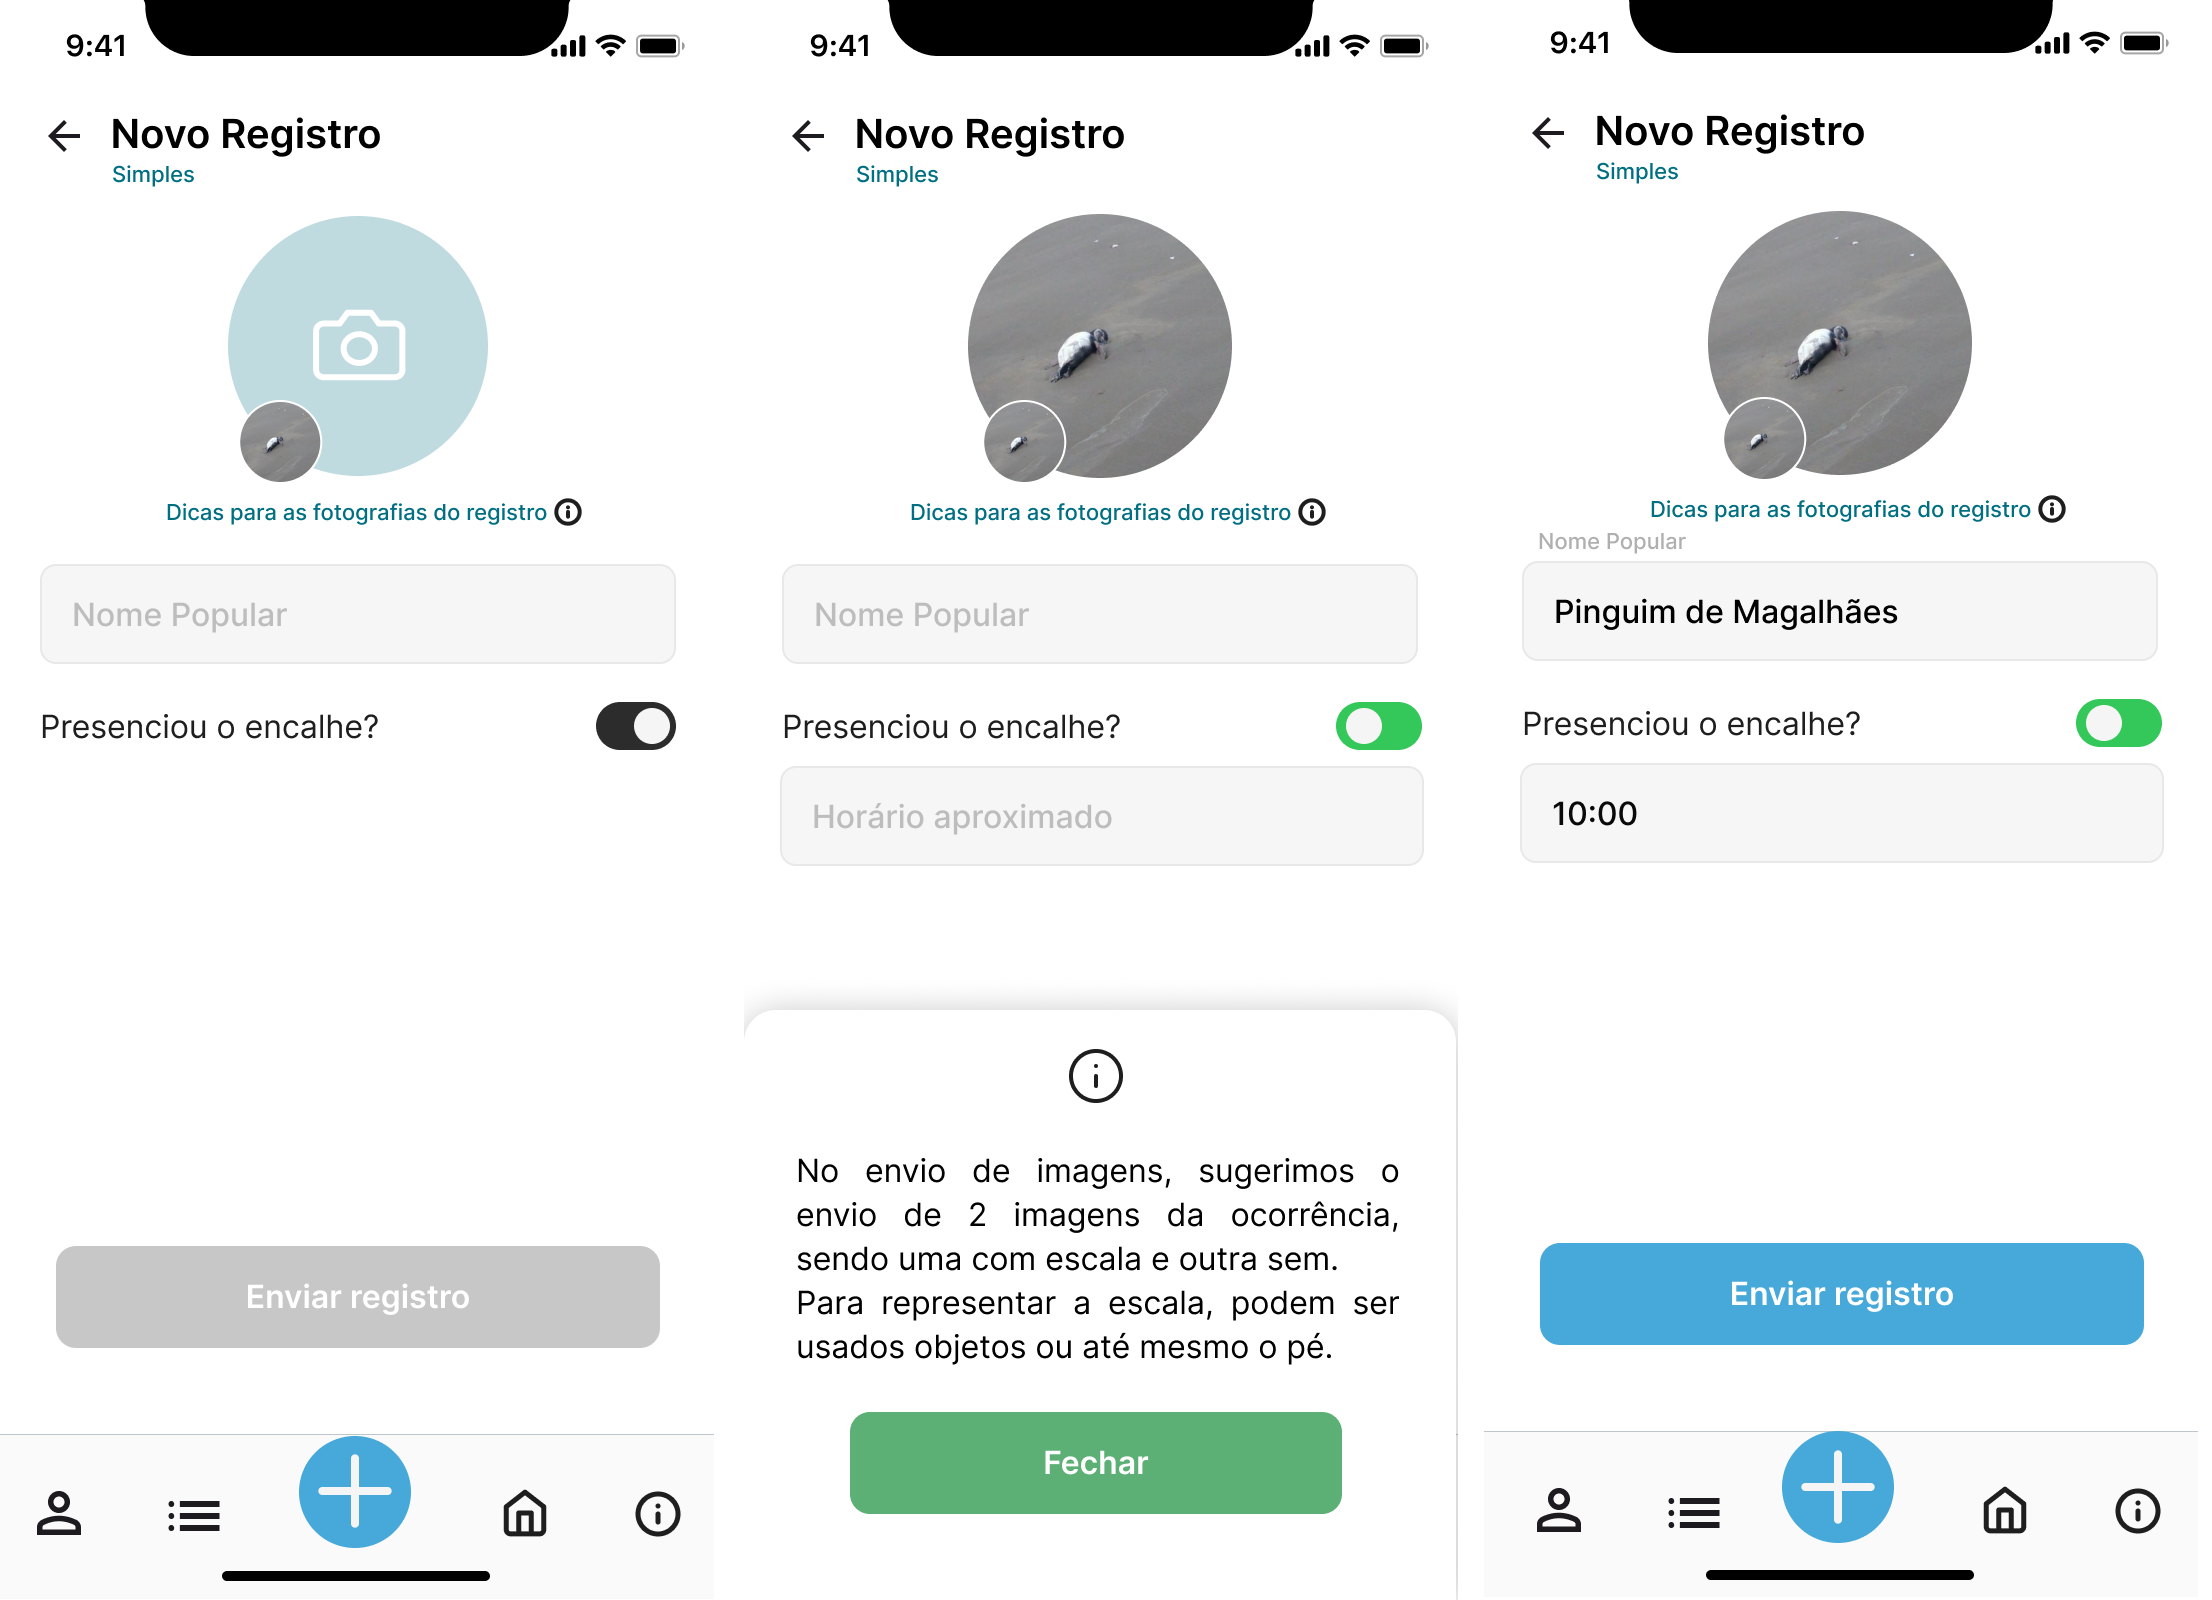
\includegraphics[height=0.55\textheight, width=\textwidth]{imagens/registro-simples-figma.png}
    \caption{Formulário de registro simples. Centro: \textit{bottomsheet} informativa; direita: campo 
    adicional ativado.}
    \label{fig:prototipo-registro-simples}
\end{figure}
\legend{Fonte: Autor}

\begin{figure}[H]
    \centering
    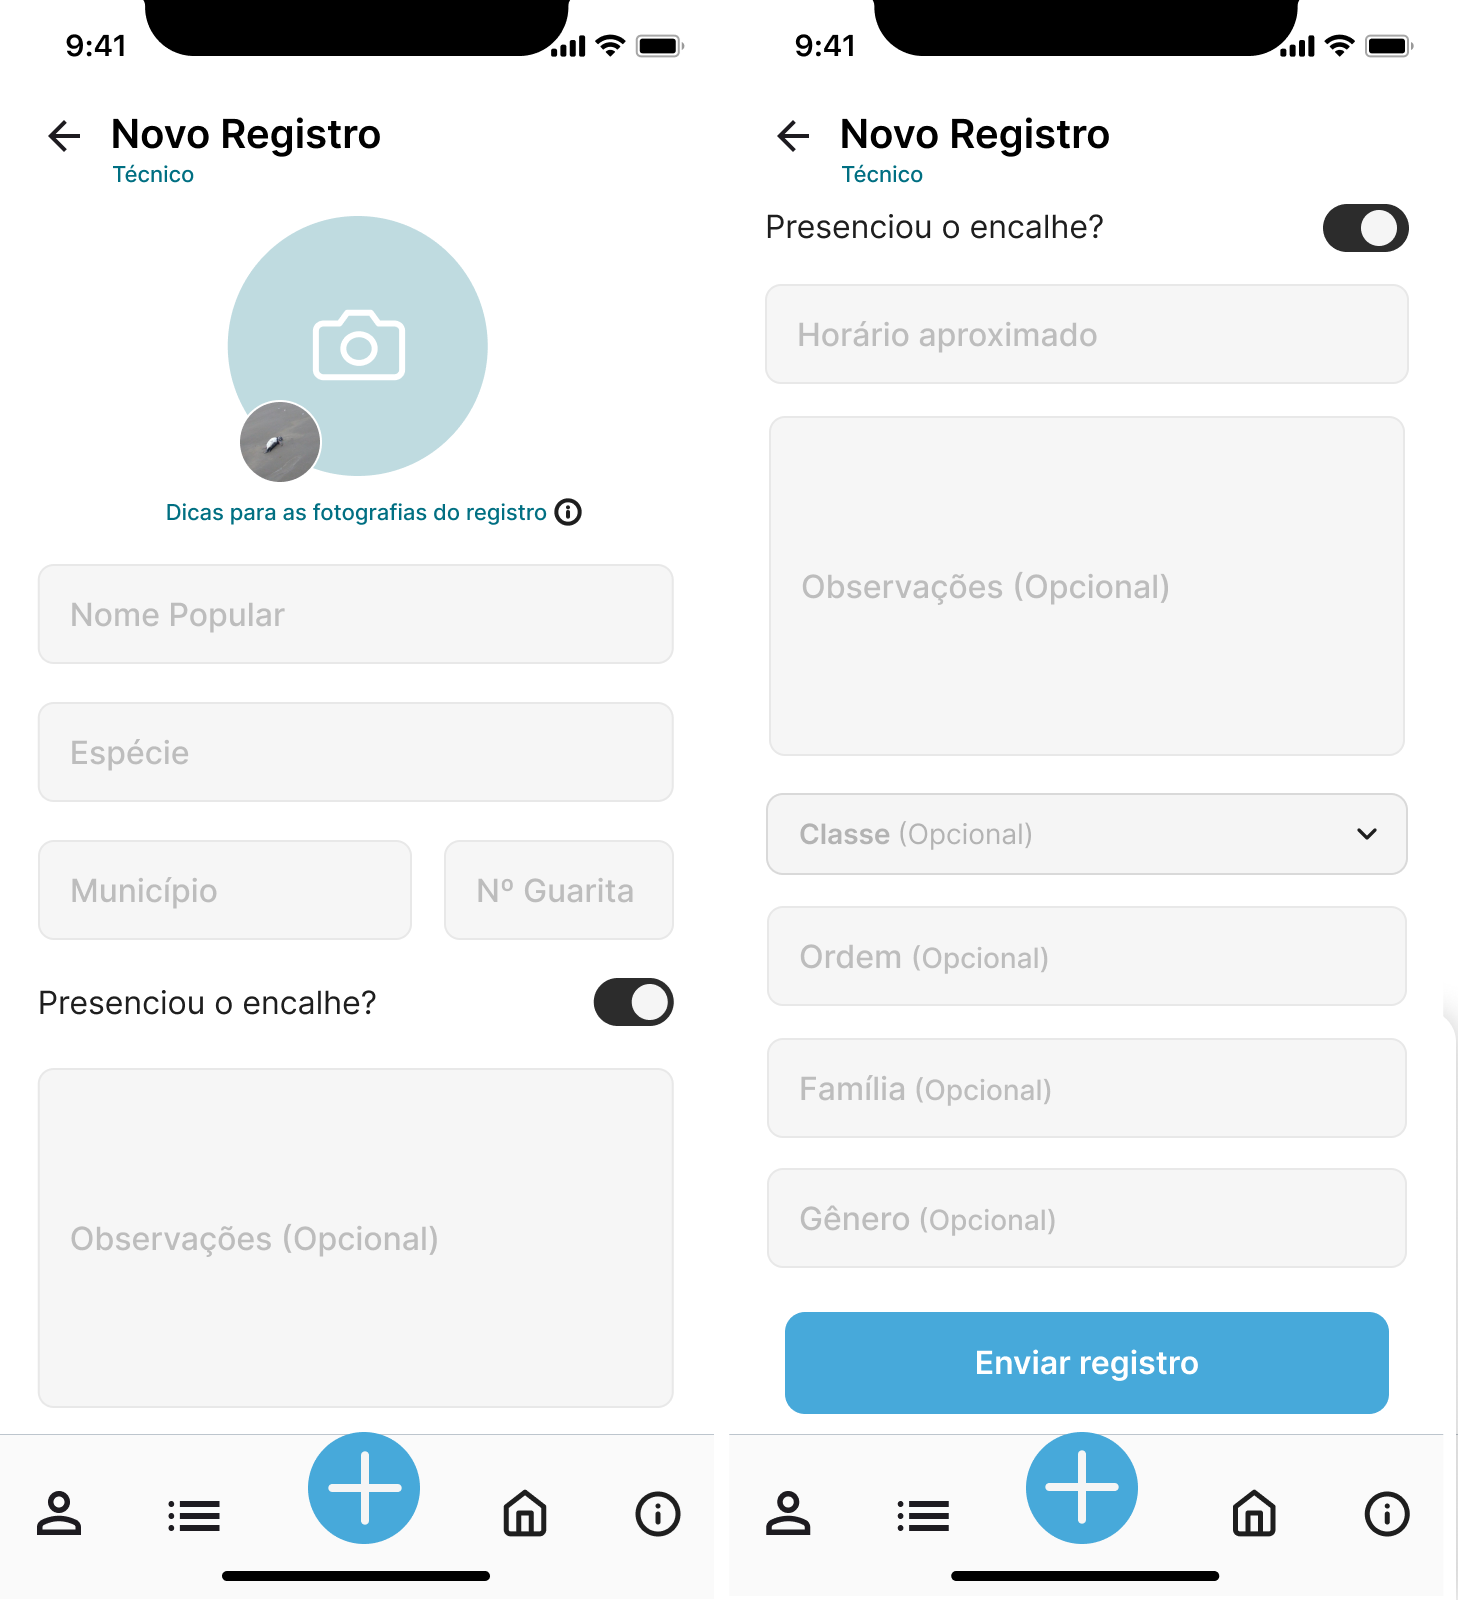
\includegraphics[height=0.6\textheight]{imagens/registro-tecnico-figma.png}
    \caption{Formulário de registro técnico com campos taxonômicos e detalhamento avançado.}
    \label{fig:prototipo-registro-tecnico}
\end{figure}
\legend{Fonte: Autor}

A tela de "Registros Pendentes" (Figura~\ref{fig:prototipo-registros-pendentes}) foi projetada 
para uso exclusivo de pesquisadores, permitindo acesso aos registros ainda não avaliados enviados 
por todos os usuários.

\begin{figure}[H]
    \centering
    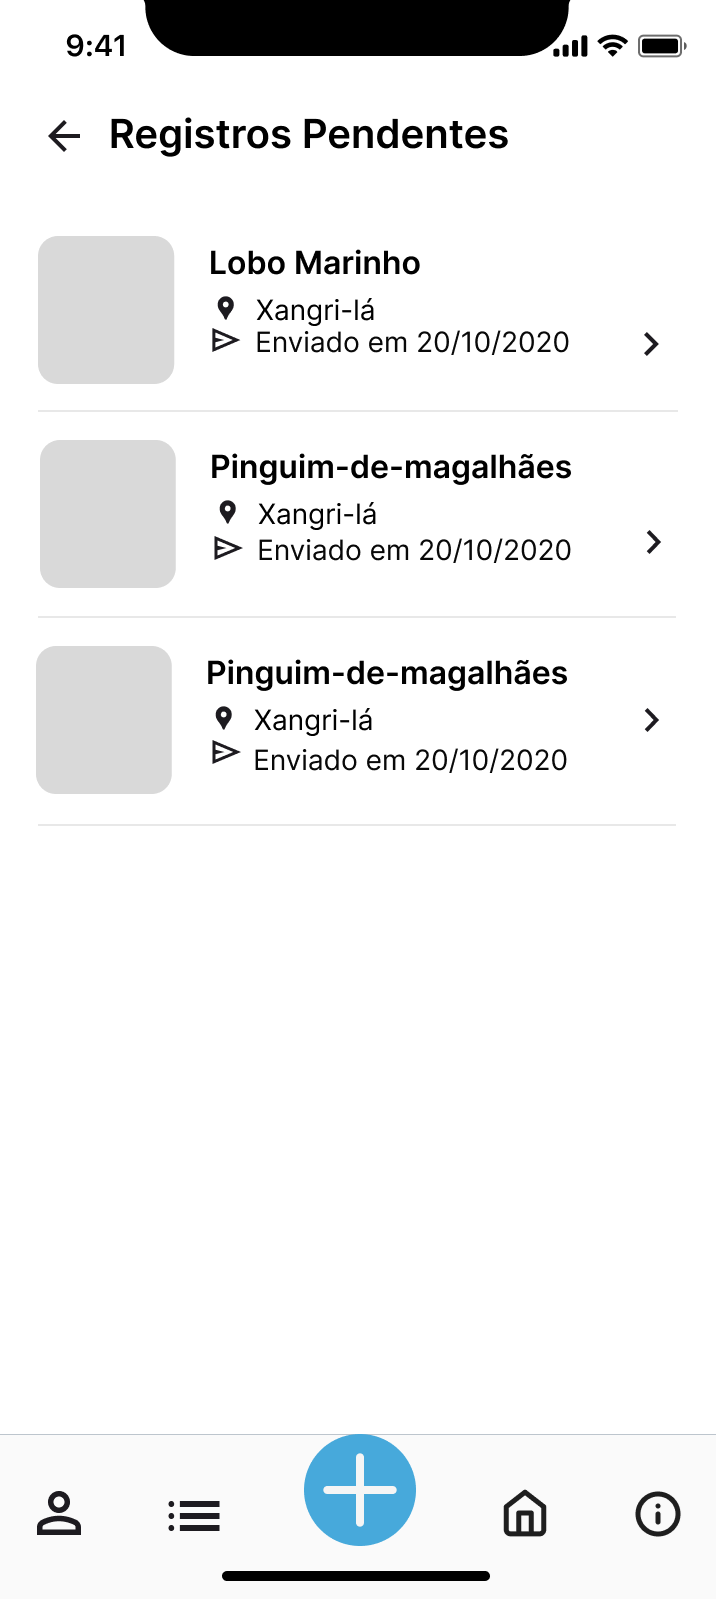
\includegraphics[height=0.6\textheight]{imagens/registro-pendente-figma.png}
    \caption{Tela de registros pendentes, acessível apenas a pesquisadores.}
    \label{fig:prototipo-registros-pendentes}
\end{figure}
\legend{Fonte: Autor}

A tela de "Analisar Registro" (Figura~\ref{fig:prototipo-avaliar-registro}) foi projetada para 
permitir que o pesquisador visualize os dados enviados em cada registro 
com a possibilidade de editar os dados, adicionar comentários e enviar uma atualização o registro.
Se fez importante adicionar um estado para esta tela, onde o pesquisador consiga selecionar a imagem
para uma visualização em tela cheia, facilitando a análise do registro.

\begin{figure}[H]
    \centering
    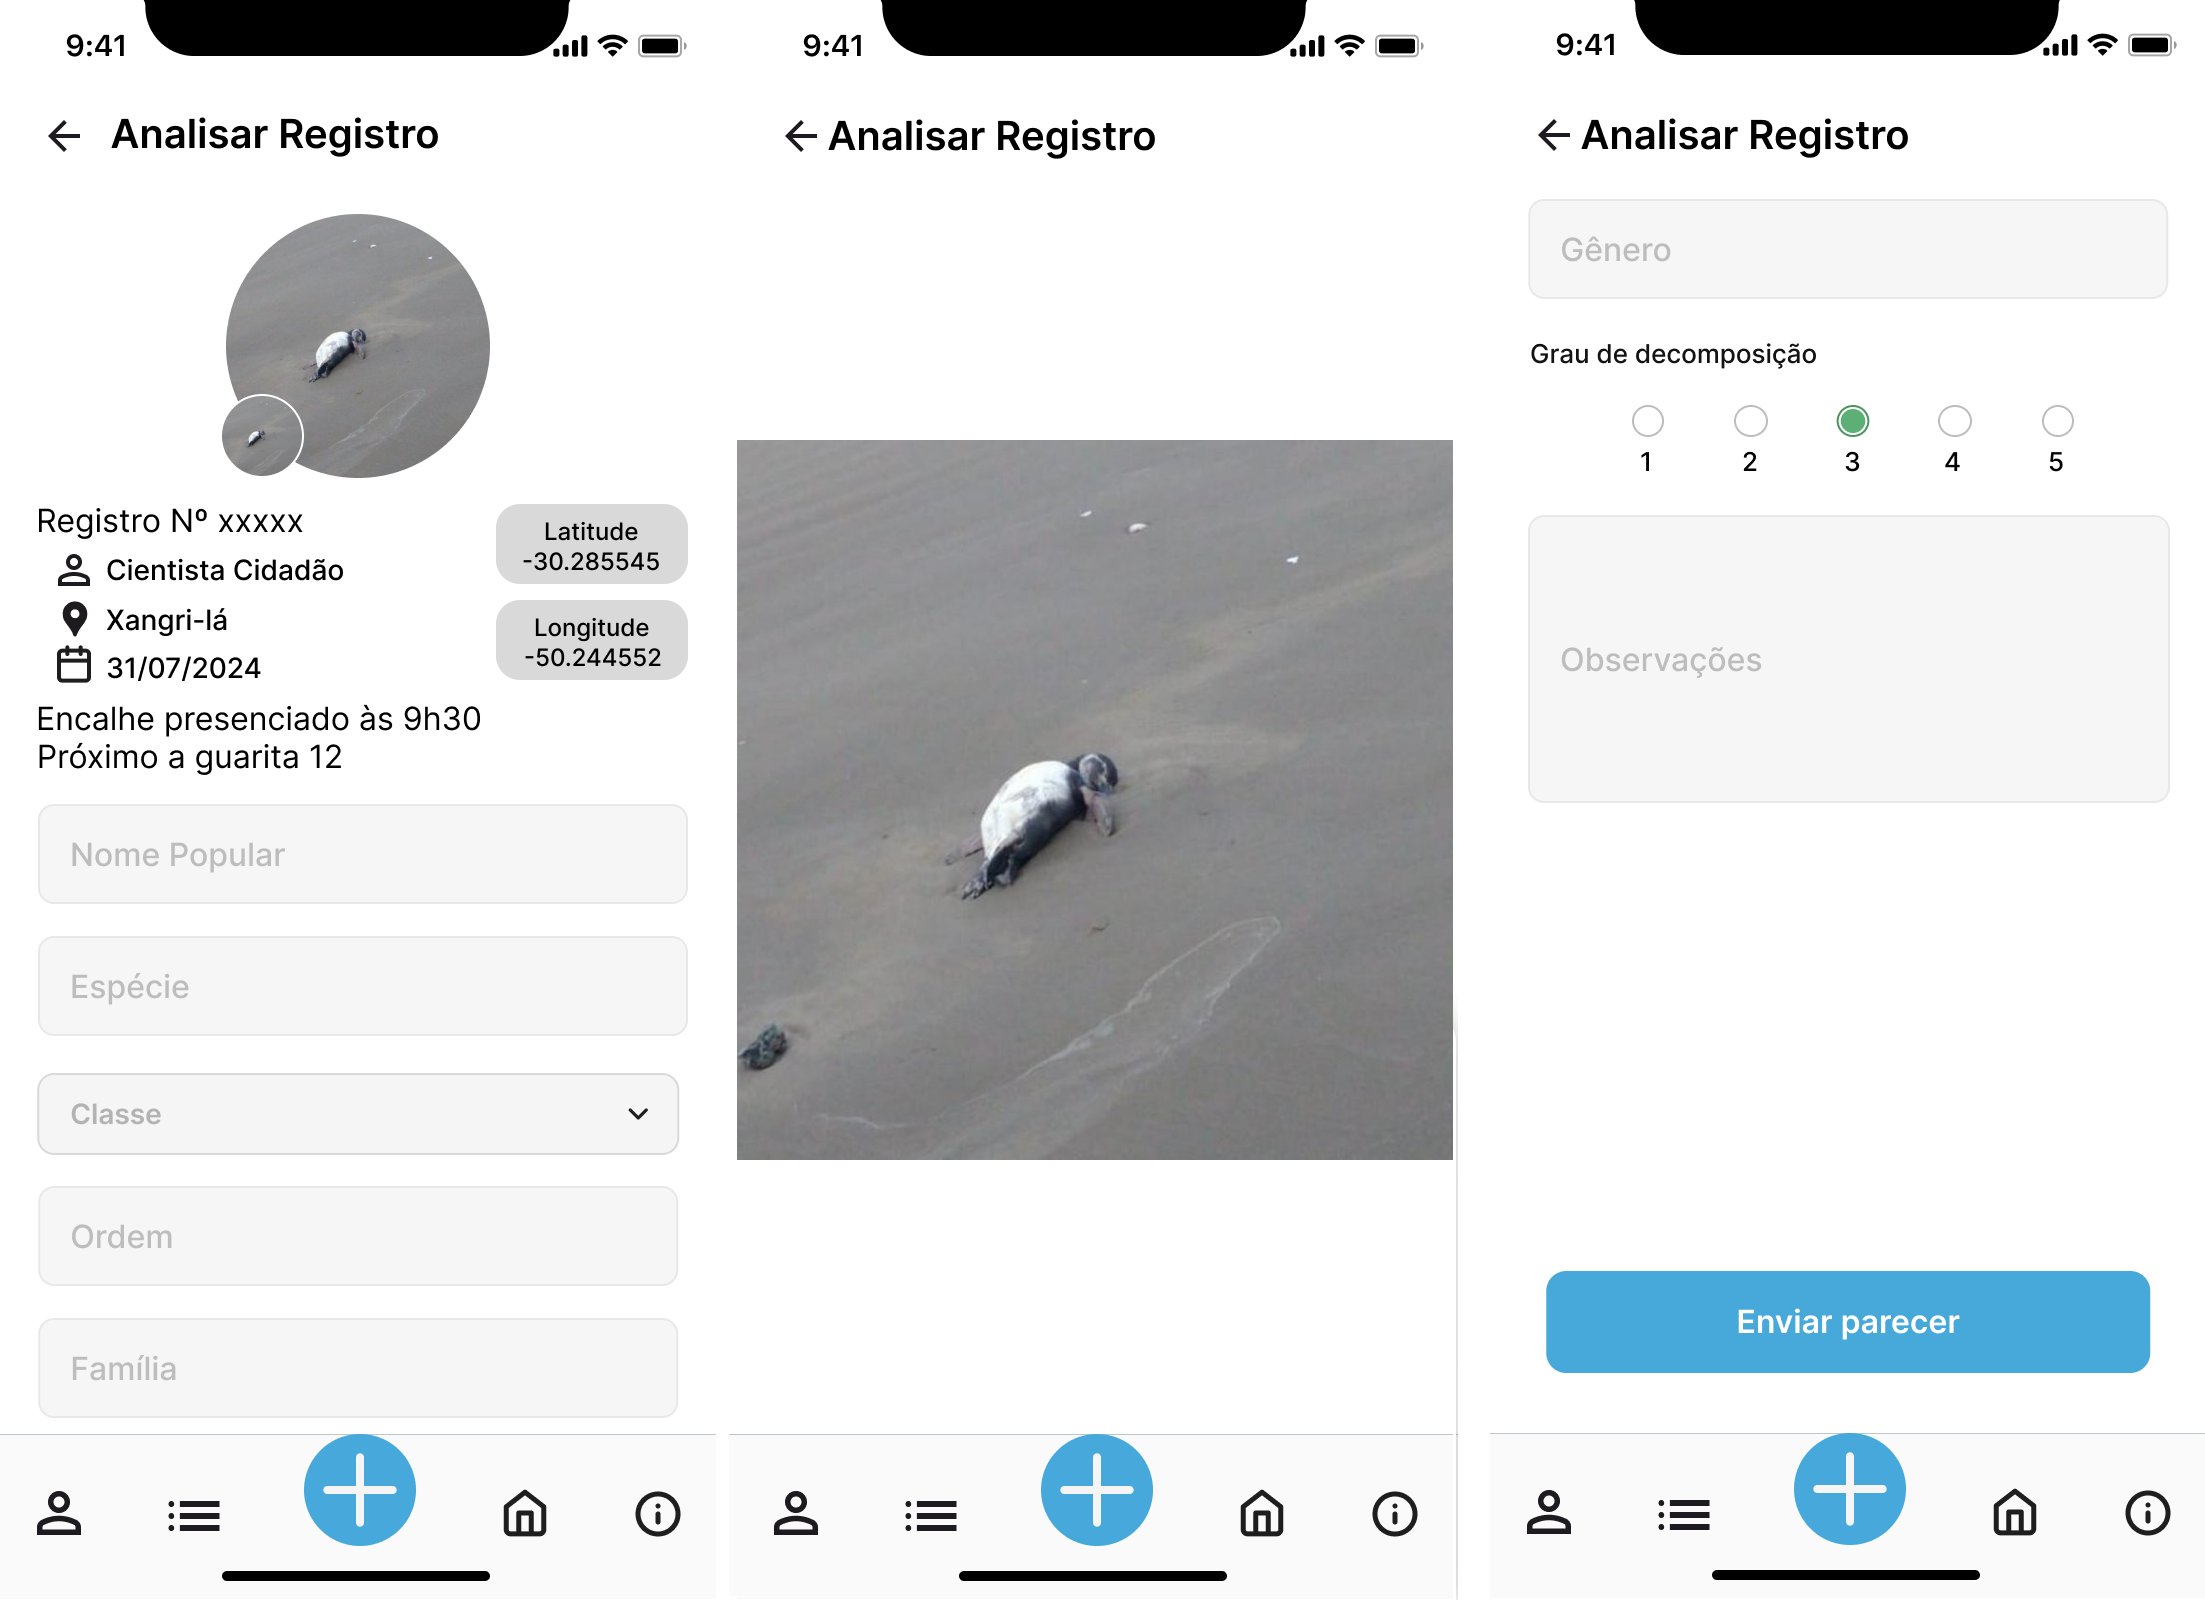
\includegraphics[height=0.55\textheight, width=\textwidth]{imagens/avaliar-registro-figma.png}
    \caption{Tela de análise de registro. Ao centro, visualização ampliada da imagem.}
    \label{fig:prototipo-avaliar-registro}
\end{figure}
\legend{Fonte: Autor}

A tela de "Visualizar Registro" foi projetada para permitir que o usuário visualize os dados
enviados e validados. Para os dados já foram validados 
(Figura~\ref{fig:prototipo-ver-registro-validado}), o registro apresentará dados extras 
sobre aquele registro, como grau de decomposição, parecer do profissional e taxonomia avaliada.
Já para os dados que ainda não foram validados (Figura~\ref{fig:prototipo-ver-registro-enviado}), 
o usuário verá apenas as informações que ele mesmo enviou.

\begin{figure}[H]
    \centering
    \begin{minipage}[b]{0.48\textwidth}
        \centering
        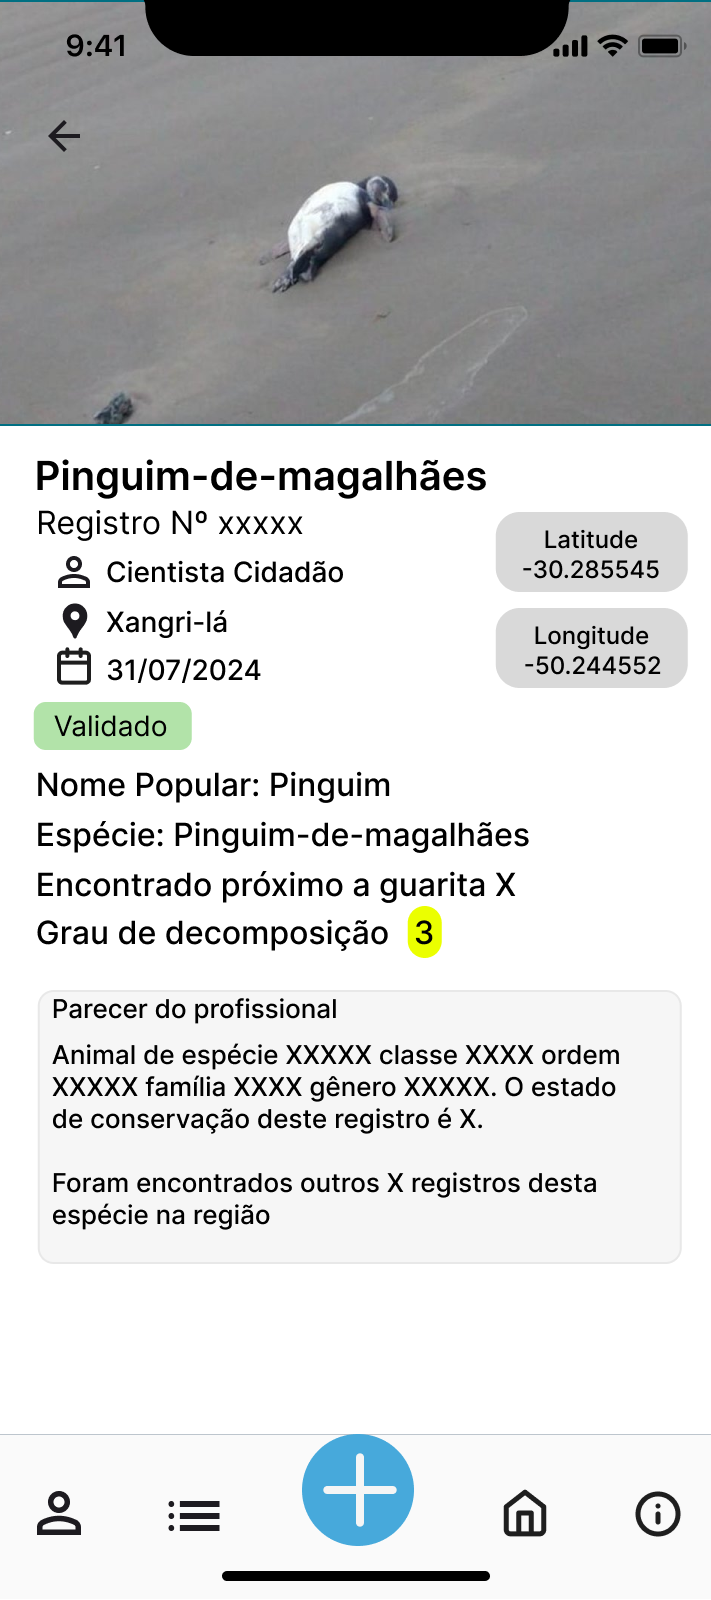
\includegraphics[height=0.6\textheight]{imagens/ver-registro-figma.png}
        \caption{Visualização de registro validado.}
        \label{fig:prototipo-ver-registro-validado}
    \end{minipage}
    \hfill
    \begin{minipage}[b]{0.48\textwidth}
        \centering
        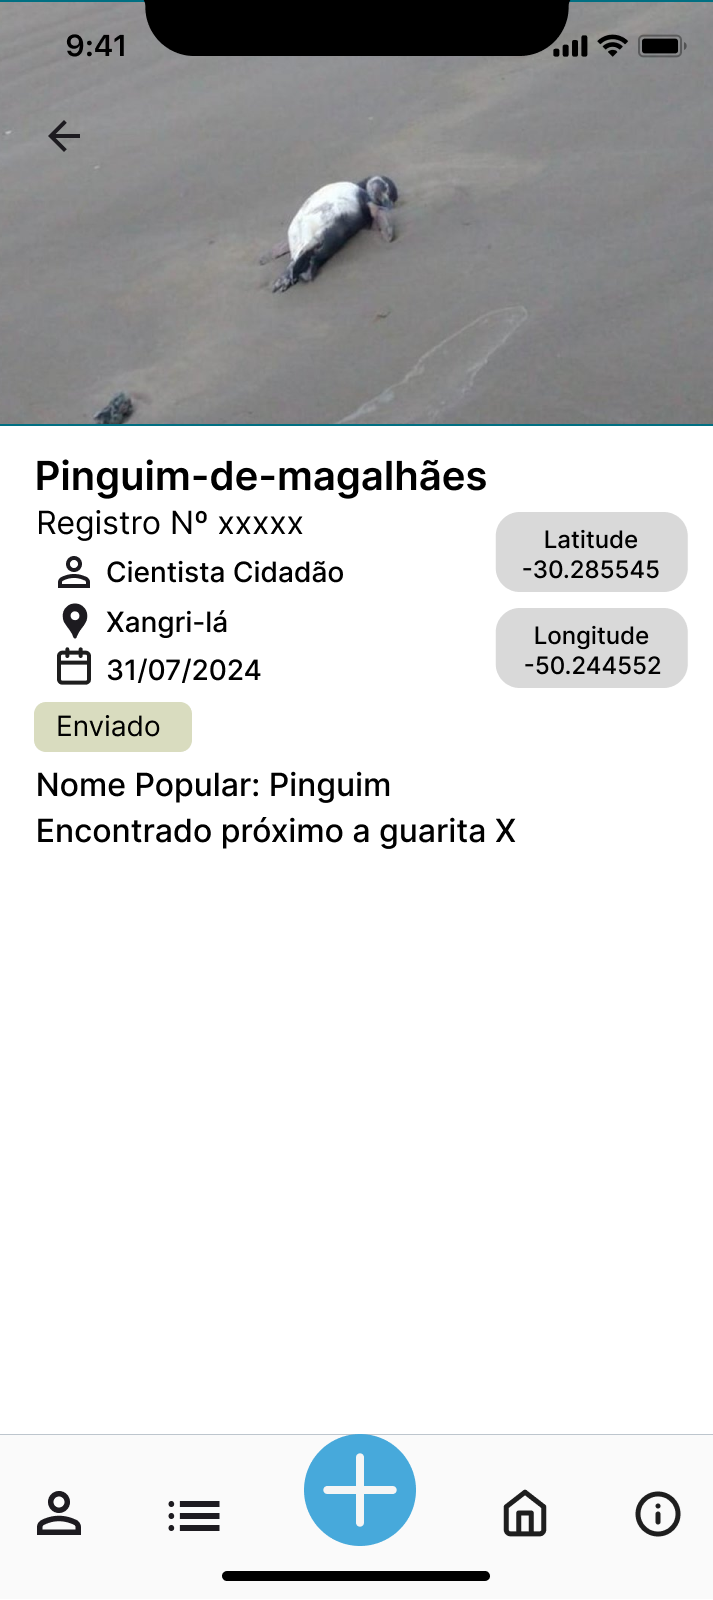
\includegraphics[height=0.6\textheight]{imagens/ve-registro-enviado-figma.png}
        \caption{Visualização de registro enviado, ainda não avaliado.}
        \label{fig:prototipo-ver-registro-enviado}
    \end{minipage}
\end{figure}
\legend{Fonte: Autor}

A tela de perfil do usuário (Figura~\ref{fig:prototipo-perfil}) apresenta dados básicos, 
quantidade de registros enviados, últimos registros e conquistas. As conquistas são exibidas 
em formato de medalhas organizadas em uma grade com três colunas.

\begin{figure}[H]
    \centering
    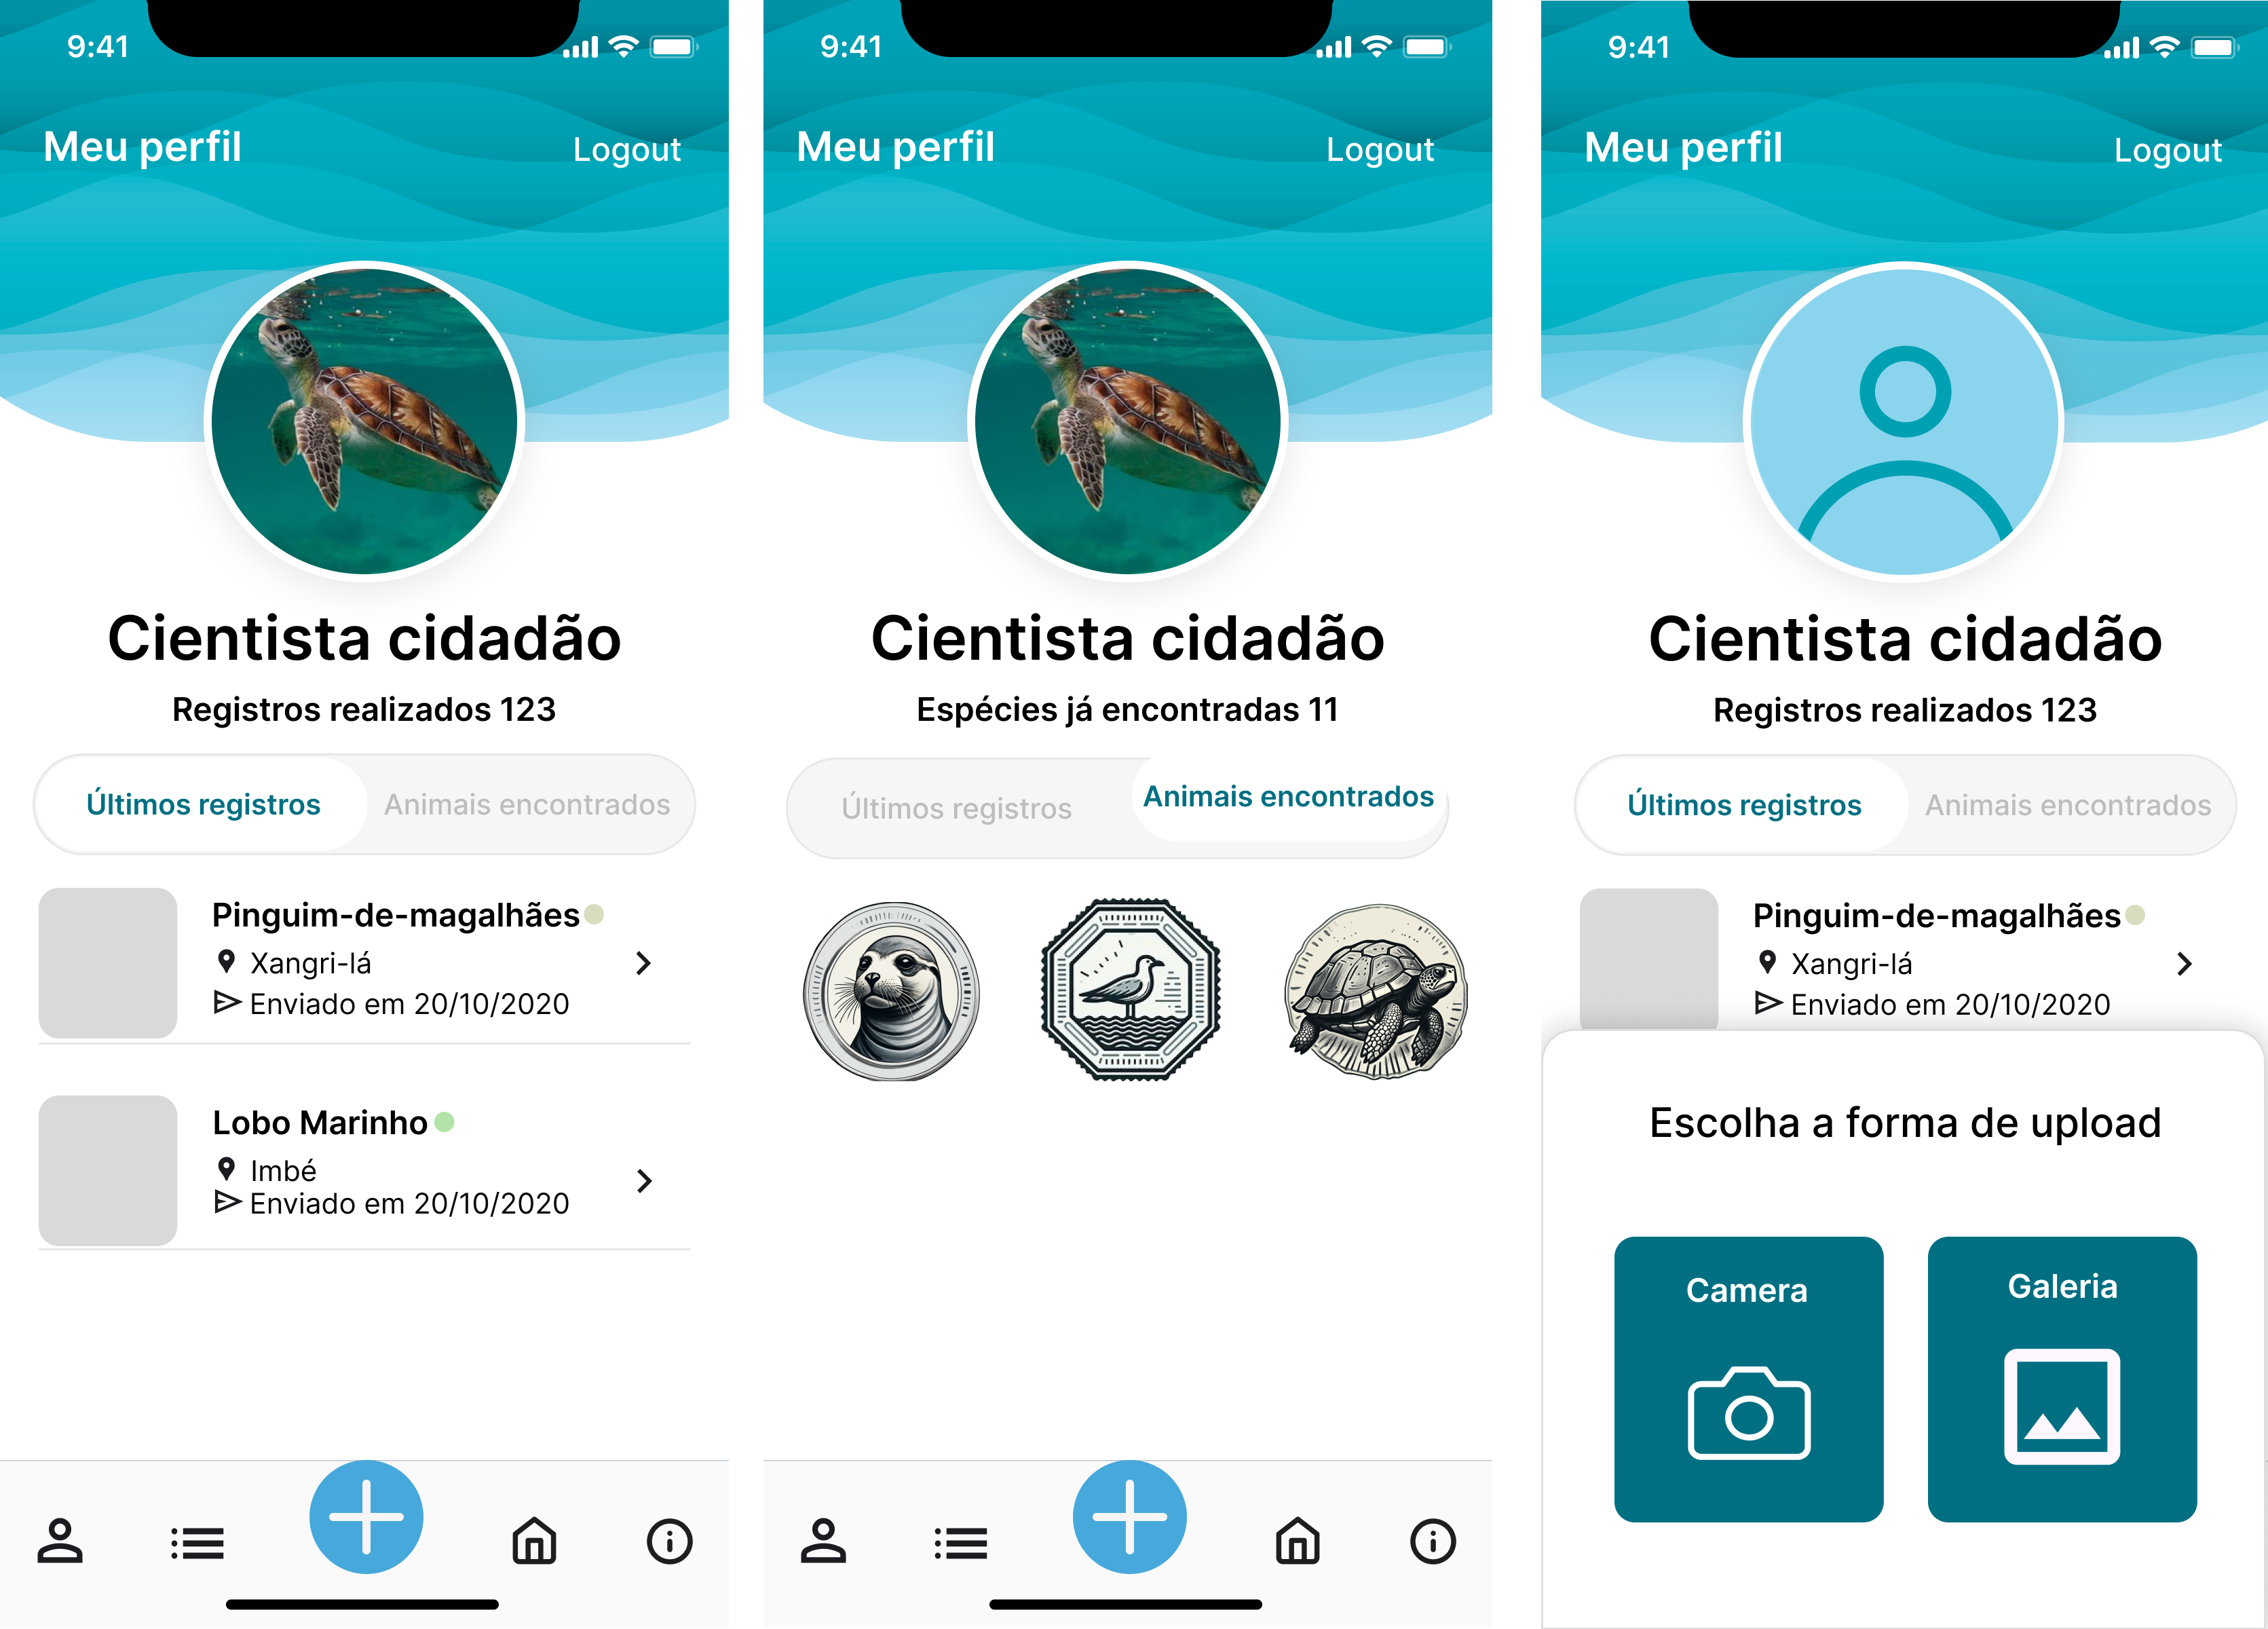
\includegraphics[height=0.53\textheight, width=\textwidth]{imagens/perfil-figma.png}
    \caption{Tela de perfil do usuário com conquistas e histórico.}
    \label{fig:prototipo-perfil}
\end{figure}
\legend{Fonte: Autor}

As telas de fauna local (Figura~\ref{fig:prototipo-fauna-local}) seguem o mesmo padrão visual 
das demais telas do aplicativo, se assemelhando em estrutura com a de "Meus Registros" e 
"Visualizar Registro". Elas apresentam, respectivamente, uma lista de espécies e uma 
tela de detalhes com informações específicas sobre cada animal que for selecionado.

\begin{figure}[H]
    \centering
    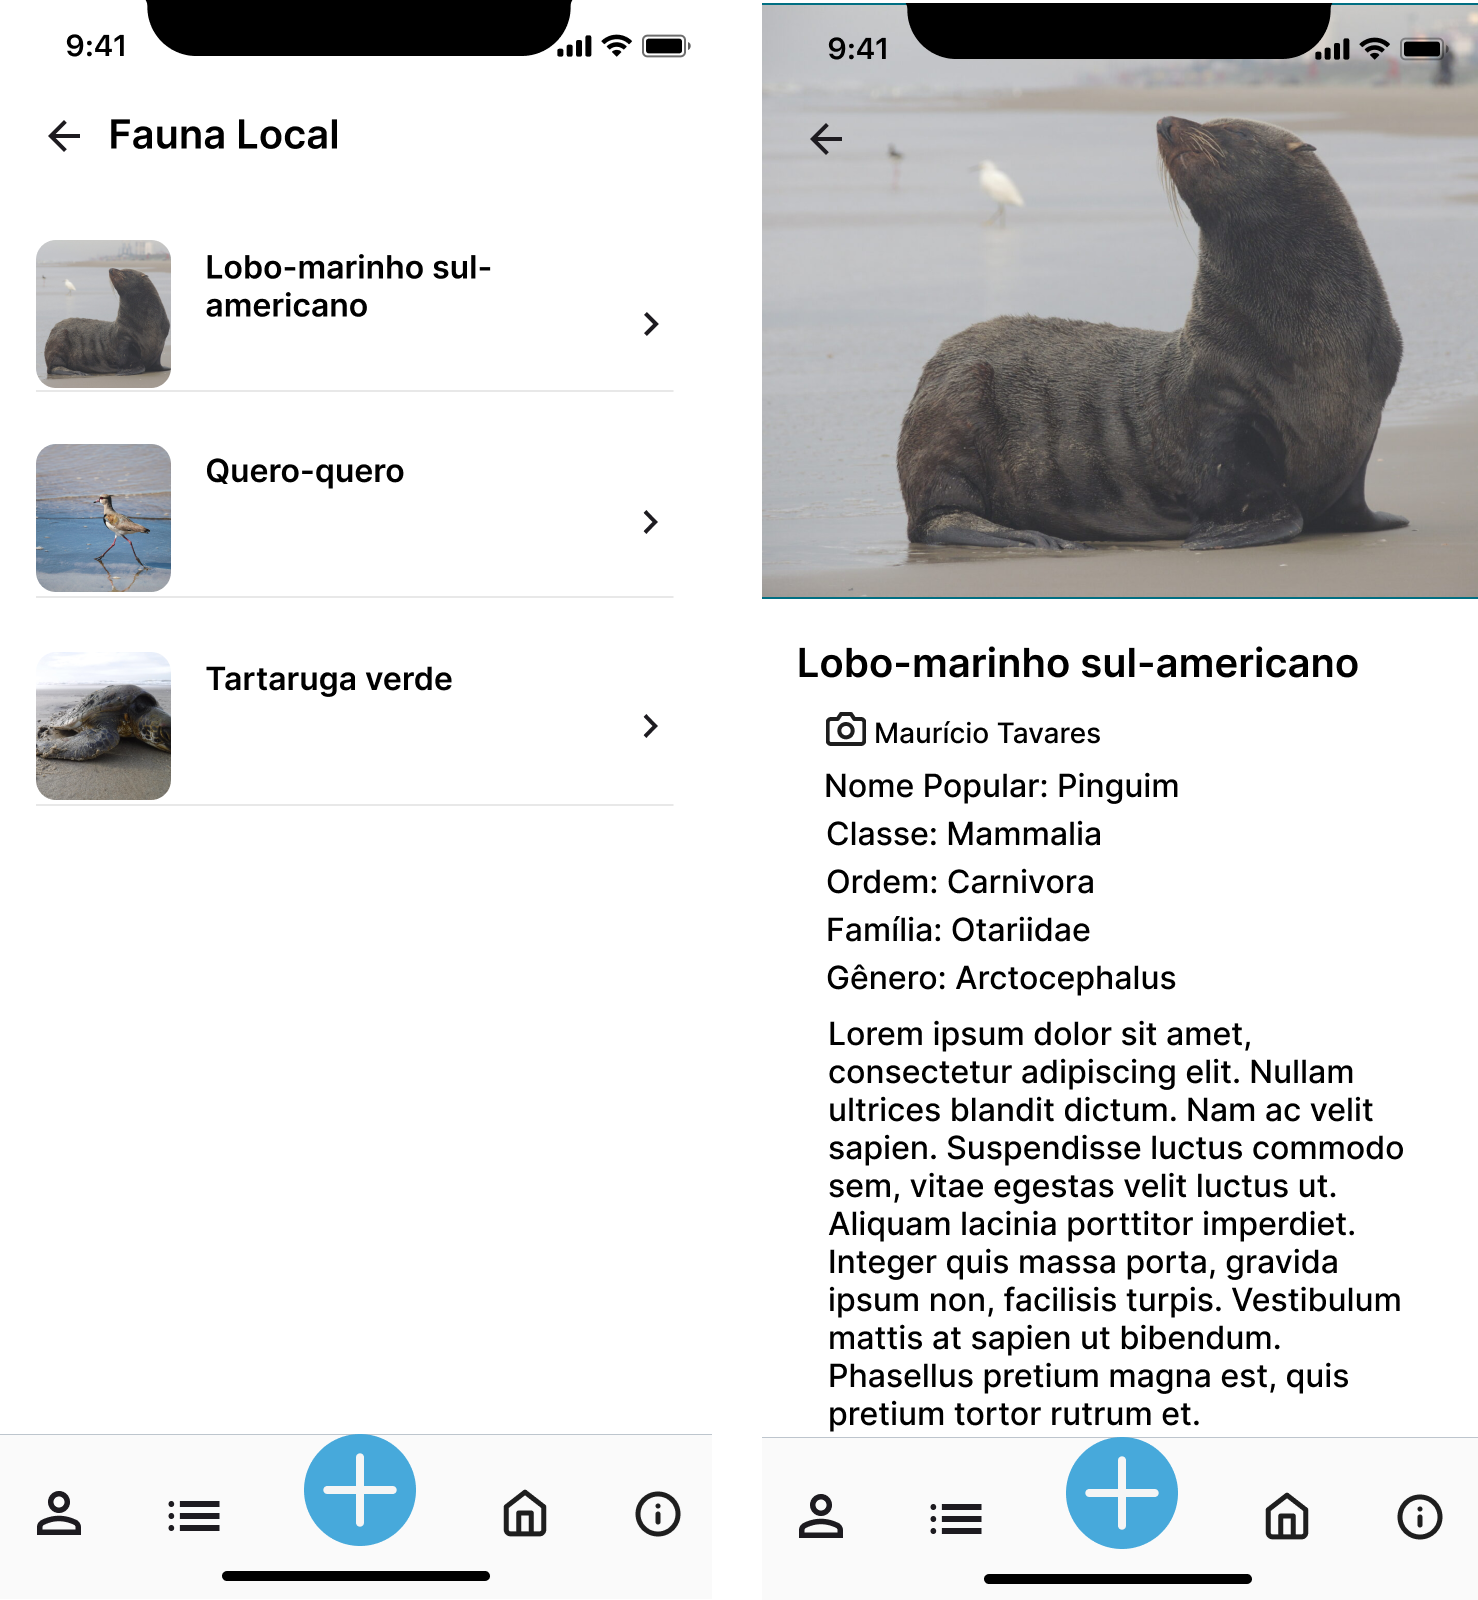
\includegraphics[height=0.6\textheight]{imagens/fauna-local-figma.png}
    \caption{Tela de fauna local (esquerda) e detalhes da espécie (direita).}
    \label{fig:prototipo-fauna-local}
\end{figure}
\legend{Fonte: Autor}

Por fim, foi projetada a tela de recuperação de senha (Figura~\ref{fig:prototipo-esqueci-senha}), 
incluindo os estados de sucesso e de erro na validação dos campos de entrada. O padrão de erro 
apresentado nesta tela foi o mesmo utilizado em outras telas do aplicativo.

\begin{figure}[H]
    \centering
    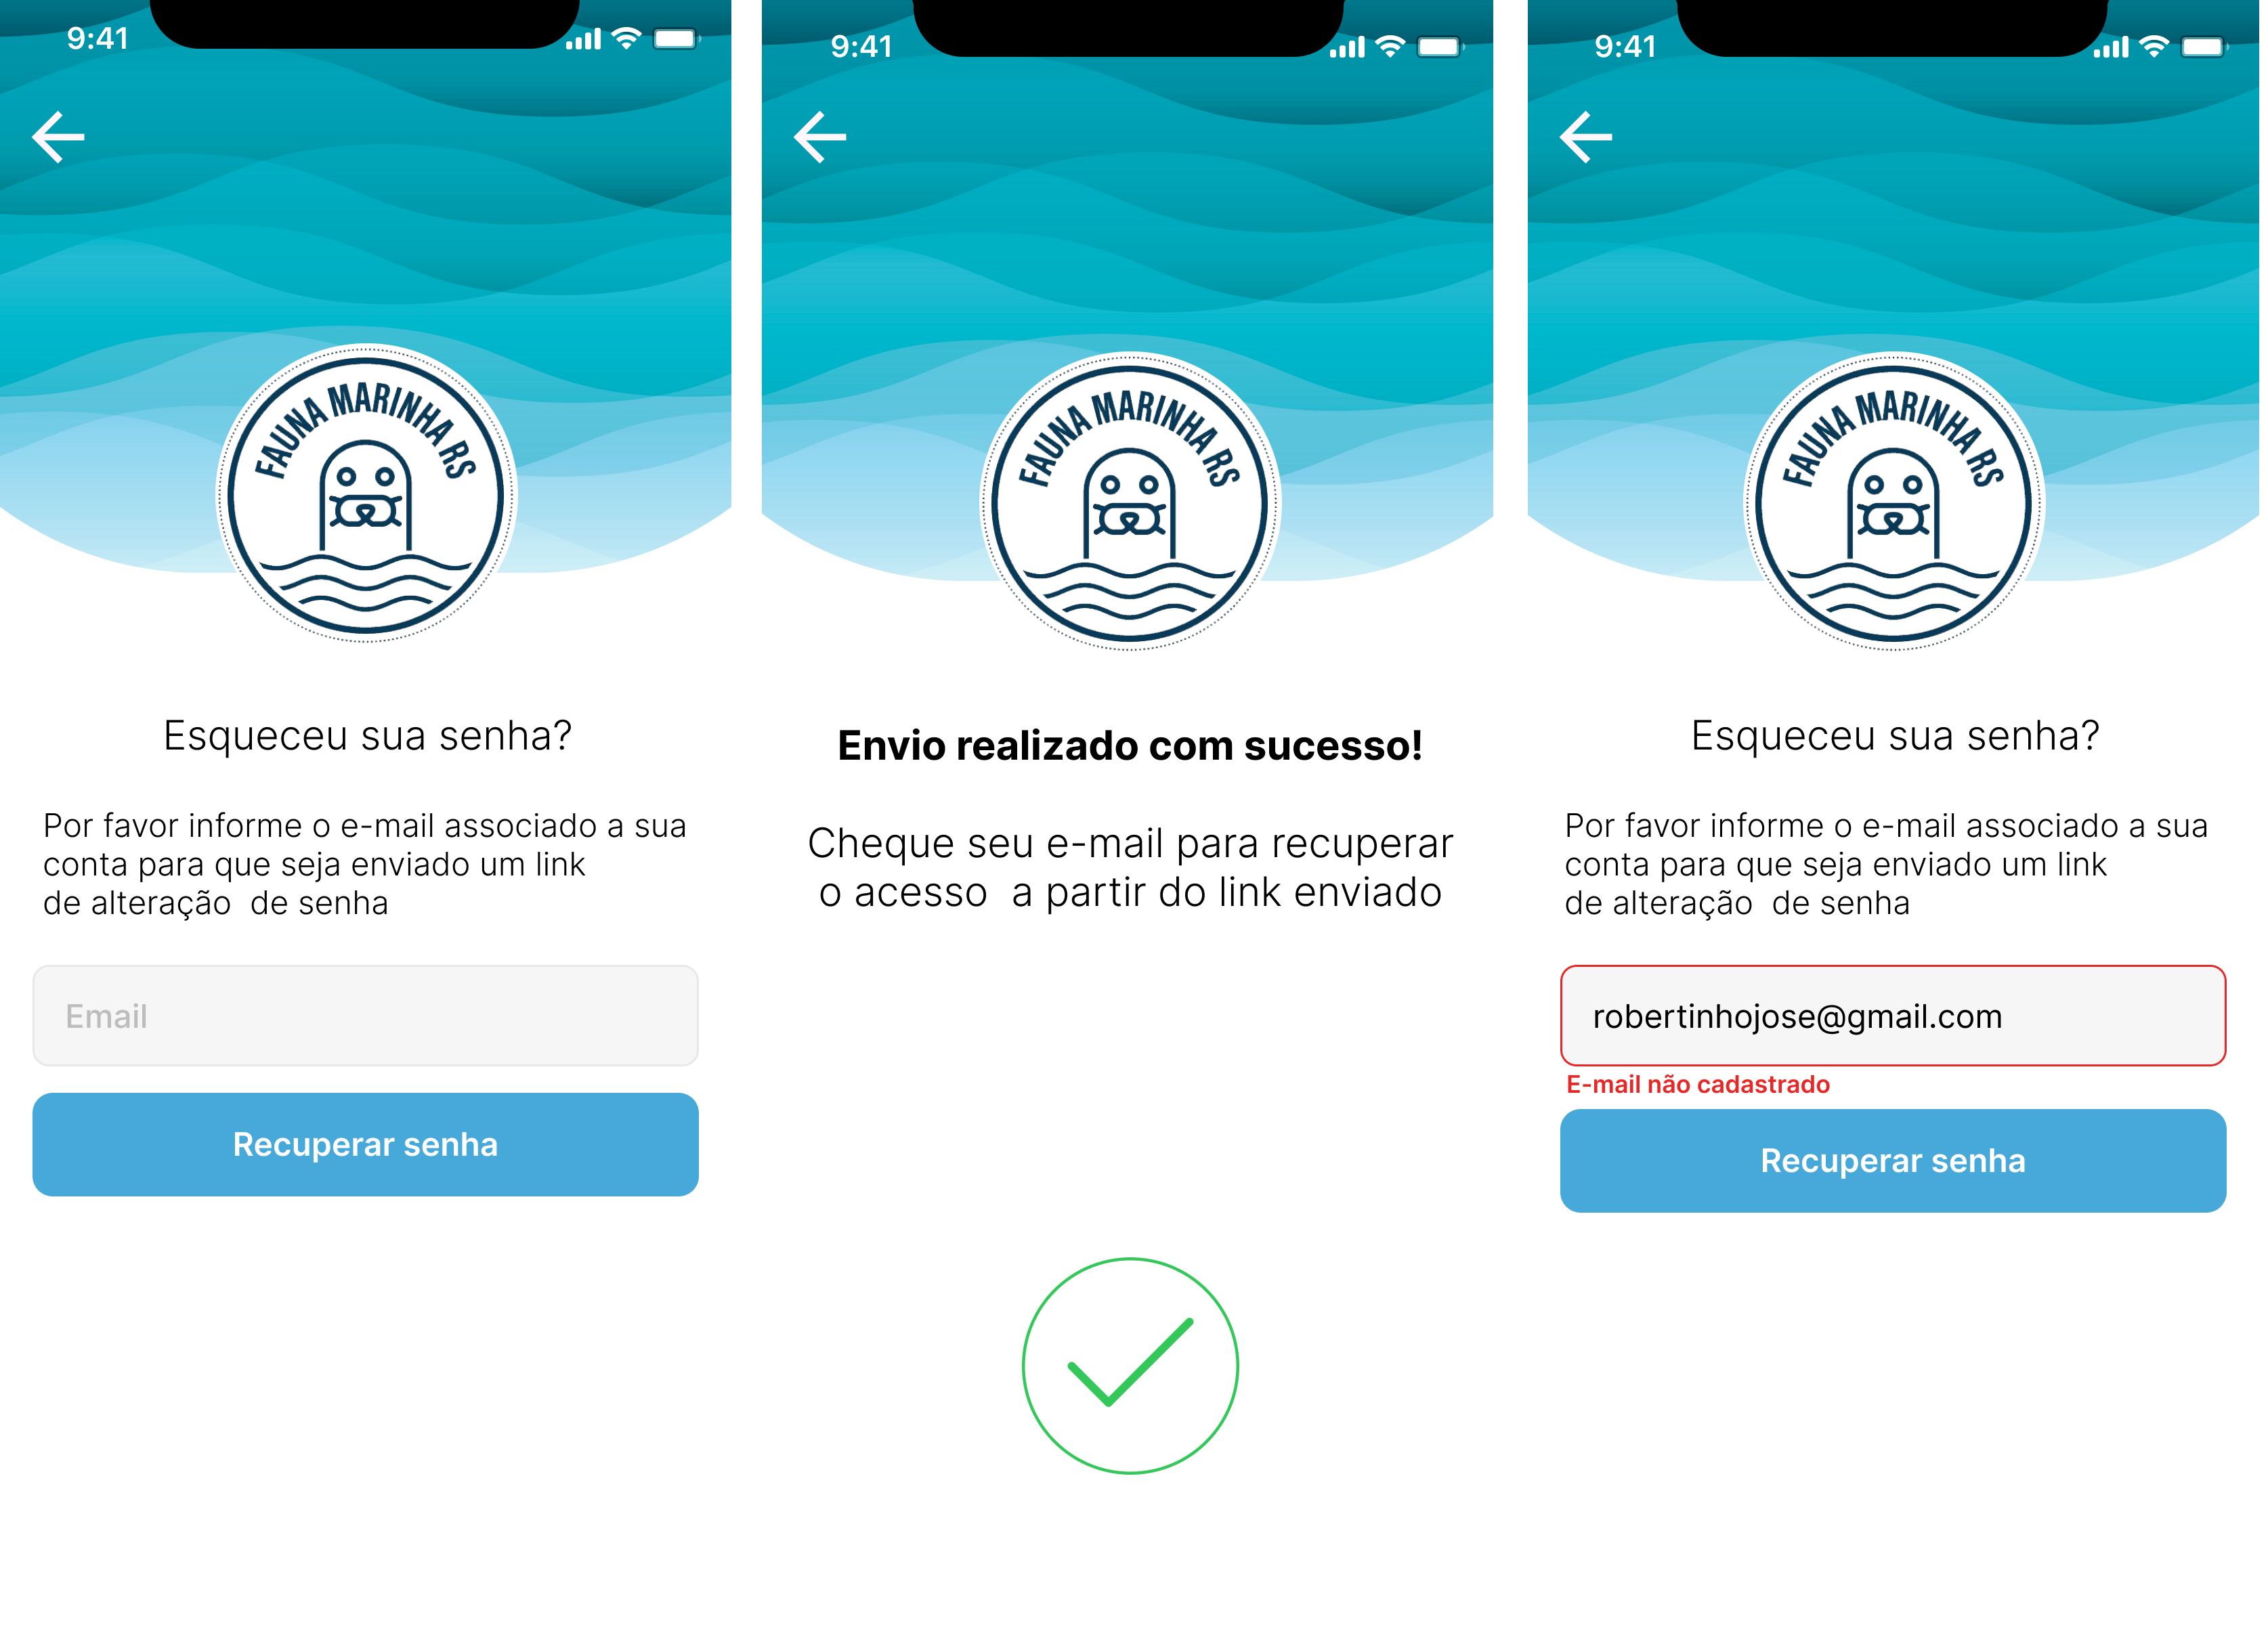
\includegraphics[height=0.53\textheight, width=\textwidth]{imagens/esqueceu-senha-figma.png}
    \caption{Tela de recuperação de senha: formulário (esquerda), sucesso (centro) e erro de 
    validação (direita).}
    \label{fig:prototipo-esqueci-senha}
\end{figure}
\legend{Fonte: Autor}

\subsection{Desenvolvimento do Protótipo Navegável}

Utilizando a ferramenta \textit{Figma} (versão gratuita \textit{online}), foi desenvolvido um
protótipo navegável de média/alta fidelidade. Essa etapa permitiu visualizar os fluxos de 
interação entre o usuário e o sistema, antecipar ajustes necessários e alinhar as funcionalidades 
às expectativas.

Foram criadas ligações interativas entre as principais telas, simulando os redirecionamentos e 
ações de navegação. O protótipo também serviu como ferramenta de validação junto a terceiros e 
como referência visual para a fase de implementação (Figura~\ref{fig:prototipo-fluxo-navegacao}).

\begin{figure}[H]
    \centering
    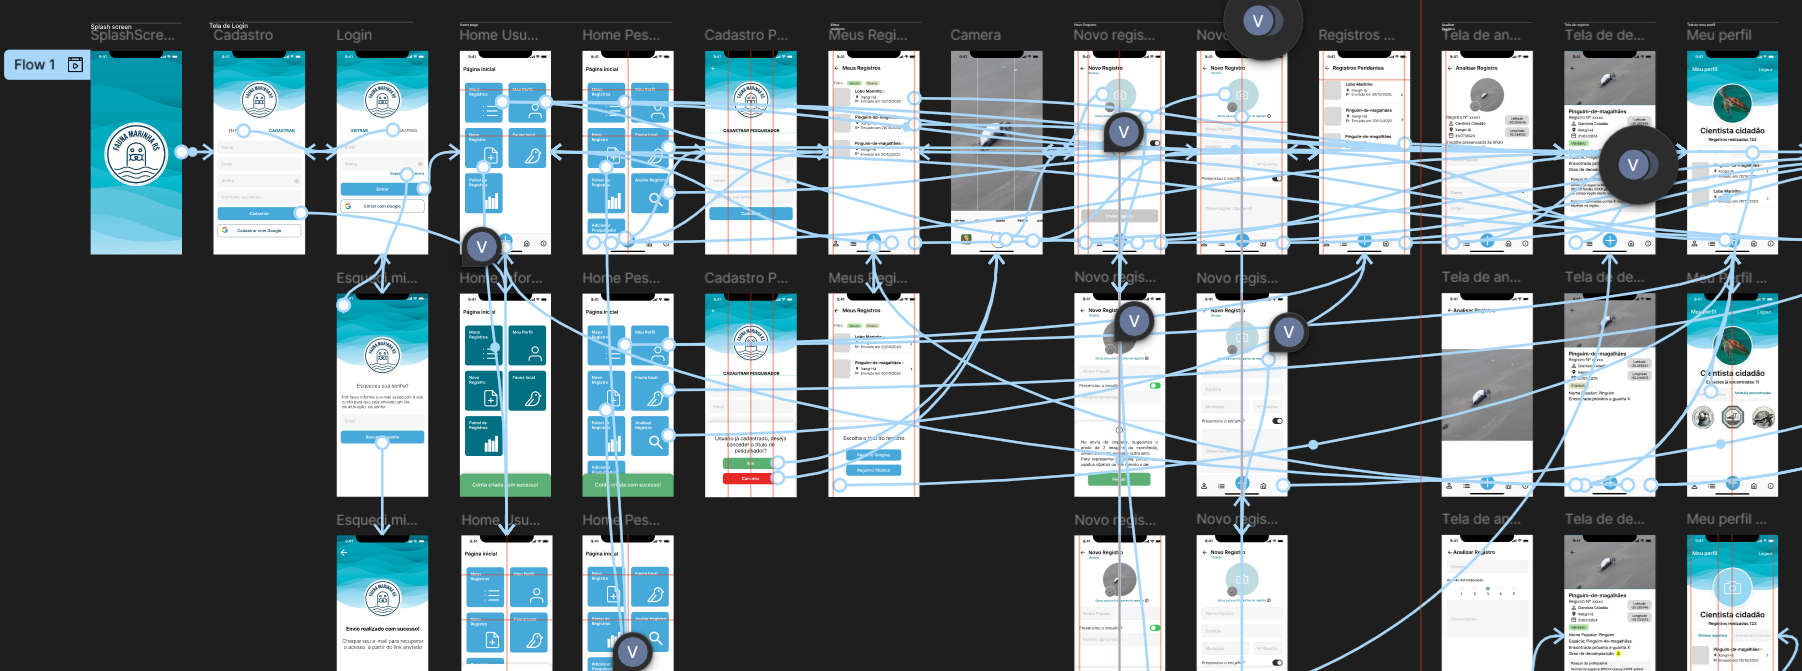
\includegraphics[width=\textwidth]{imagens/prototipo-navegavel-figma.png}
    \caption{Captura de tela do protótipo navegável desenvolvido no \textit{Figma}.}
    \label{fig:prototipo-fluxo-navegacao}
\end{figure}
\legend{Fonte: Autor}

\section{Projeto Gerencial}
% descrever o fluxo de trabalho documentado no Jira, com cards
A gerência desse projeto foi realizada utilizando a ferramenta \textit{Jira}, que possibilitou o
controle de tarefas e o acompanhamento do progresso do desenvolvimento. O fluxo de trabalho
descrito na \hyperref[sec:metodologia-desenv-software]{Seção de metodologia} deste trabalho foi 
seguido para garantir a organização e a eficiência
das tarefas. Os \textit{cards} gerados no \textit{board} foram puxados para trabalho a medida que 
havia tempo disponível para atuação. Foram catalogadas não só tarefas de codificação, como 
também tarefas de prototipação.

Foram gerados ao todo, 131 \textit{cards} desde julho de 2024 quando se deu inicio a prototipação 
da aplicação. Na Figura \ref{gra:cards-mes} é possível observar a quantidade de itens no eixo vertical
relacionada com o mês de criação no eixo horizontal. Com ele podemos concluir que os meses com 
mais entrada de demandas foram os meses de novembro de 2024, janeiro de 2025 e março de 2025,
onde o número de \textit{cards} criados foi maior que 18.

\begin{figure}[H]
    \centering
    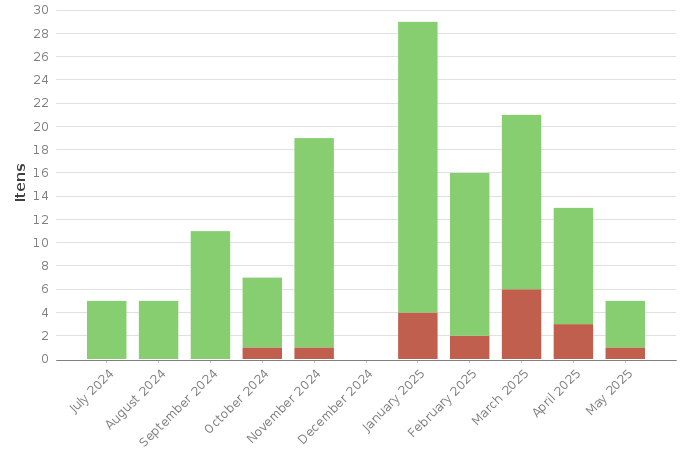
\includegraphics[width=\textwidth]{imagens/itensMes.png}
    \caption{Gráfico demonstrativo de \textit{cards} criados por mês no \textit{Jira}. As 
    barras em verde representam demandas que, até a data de criação do gráfico, já haviam sido finalizadas.
    As barras em vermelho representam demandas que ainda estavam em aberto.}
    \label{gra:cards-mes}
\end{figure}
\legend{Fonte: Autor}

A Figura \ref{gra:cards-vs-resolvidos} traz uma visão cumulativa do trabalho realizado no board.
A partir dele podemos ver que, dos 131 cards criados, 113 foram concluídos, o que representa 86,26\% 
do total. Podemos observar também que, em momentos de maior atuação no projeto, a criação de 
cards está diretamente relacionada com a quantidade de cards resolvidos.
Isso está principalmente relacionado com a disponibilidade de tempo para atuar no projeto, e também
com a criação de bugs e novas demandas que surgiram durante o desenvolvimento.

\begin{figure}[H]
    \centering
    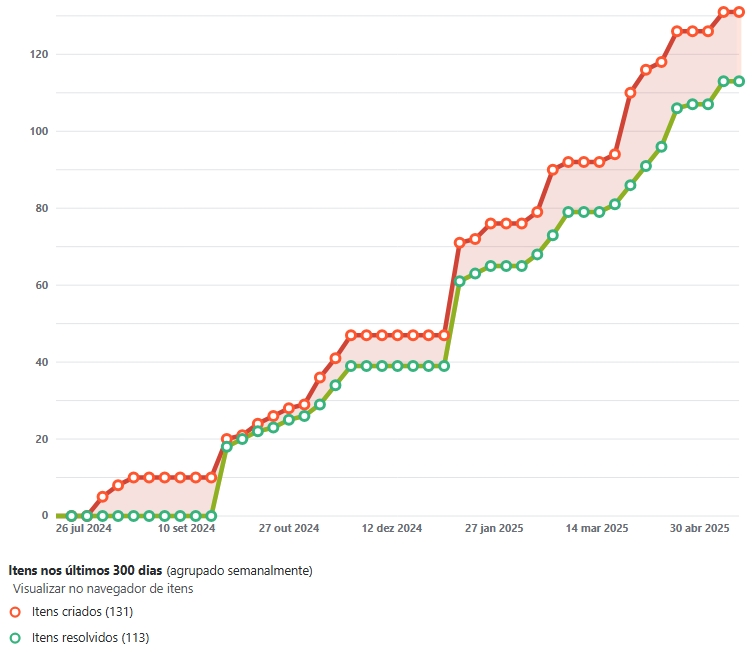
\includegraphics[width=\textwidth]{imagens/burnup-jira.jpeg}
    \caption{Gráfico demonstrativo de \textit{cards} vs resolvidos no \textit{Jira}}
    \label{gra:cards-vs-resolvidos}
\end{figure}
\legend{Fonte: Autor}

A Figura~\ref{gra:tempo-medio-resolucao} apresenta o tempo médio, em dias, 
para a resolução dos \textit{cards} ao longo das semanas. É possível notar uma grande variação 
nos tempos médios, com valores baixos no período de novembro e um pico em maio de 2025. 
Esse aumento progressivo reflete a falta de atuação evidenciada no mês de dezembro vide 
Figura\ref{gra:cards-vs-resolvidos}, o aumento na complexidade das demandas e o acumulo de 
cards de melhoria no \textit{Backlog} que foram criados e não priorizados.

\begin{figure}[H]
    \centering
    \includegraphics[width=\textwidth]{imagens/tempo-médio-cards.png}
    \caption{Gráfico demonstrativo de tempo de resolução médio dos \textit{cards} por semana no \textit{Jira}}
    \label{gra:tempo-medio-resolucao}
\end{figure}
\legend{Fonte: Autor}

Os \textit{cards} foram organizados em três grupos principais, que representam as diferentes
atuações necessárias para atuar em cada uma delas.
\subsection{Desenvolvimento Geral}
Esses cards representam demandas que passaram por etapas de planejamento e refinamento, 
refletindo as histórias de usuário e tarefas técnicas previstas ou requisitadas durante o desenvolvimento.
A Tabela~\ref{tab:desenv_geral_sorted} apresenta esse conjunto de funcionalidades. Ao todo foram 66 demandas
send 62 concluídas e 4 que ainda estão no \textit{Backlog}.

% manter essa tabela aqui ou colocar no anexo?
% talvez isso deveria ser um anexo? 

\begin{longtable}{@{}lp{7cm}ll@{}}
\caption{Registro de desenvolvimento geral (Ordenado por Data de Entrega)}\label{tab:desenv_geral_sorted}\\
\toprule
\textbf{Chave} & \textbf{Resumo} & \textbf{Status} & \textbf{Entregue} \\
\midrule
\endfirsthead

\caption{(Continuação) Registro de desenvolvimento geral (Ordenado por Data de Entrega)}\\
\toprule
\textbf{Chave} & \textbf{Resumo} & \textbf{Status} & \textbf{Entregue} \\
\midrule
\endhead

\midrule
\multicolumn{4}{r@{}}{(Continua na próxima página)} \\
\endfoot

\bottomrule
\endlastfoot

CEC-1 & Prototipação inicial das telas & Concluído & 2024-09-27 \\
CEC-2 & Tela de registro & Concluído & 2024-09-27 \\
CEC-3 & Tela de login & Concluído & 2024-09-27 \\
CEC-4 & Tela de novo registro Simples & Concluído & 2024-09-27 \\
CEC-5 & Tela de meus registros & Concluído & 2024-09-27 \\
CEC-6 & Tela de Coletanea animais & Concluído & 2024-09-27 \\
CEC-7 & Tela de perfil do usuário & Concluído & 2024-09-27 \\
CEC-8 & Tela de adicionar pesquisador & Concluído & 2024-09-27 \\
CEC-9 & Tela de esqueci minha senha & Concluído & 2024-09-27 \\
CEC-10 & Tela de selos de conquista & Concluído & 2024-09-27 \\
CEC-11 & Tela de novo registro Técnico & Concluído & 2024-09-27 \\
CEC-12 & Tela de home & Concluído & 2024-09-27 \\
CEC-13 & Tela de analisar Registro & Concluído & 2024-09-27 \\
CEC-14 & Tela de SplashScreen & Concluído & 2024-09-27 \\
CEC-15 & Tela sobre o app & Concluído & 2024-09-27 \\
CEC-16 & Codificação da SplashScreen & Concluído & 2024-09-27 \\
CEC-17 & Codificação da Tela de Registro & Concluído & 2024-09-28 \\
CEC-18 & Codificação da Tela de Login & Concluído & 2024-09-28 \\
CEC-21 & Codificação esqueci minha senha & Concluído & 2024-09-29 \\
CEC-20 & Codificação da Tela de Cadastrar Pesquisador & Concluído & 2024-10-03 \\
CEC-19 & Codificação da HomePage & Concluído & 2024-10-07 \\
CEC-22 & Adição funcionalidade de adicionar novo registro + bottom sheet & Concluído & 2024-10-09 \\
CEC-23 & Tela de registro simples & Concluído & 2024-10-15 \\
CEC-24 & Tela de registro tecnico & Concluído & 2024-10-21 \\
CEC-25 & Tela de registro controller & Concluído & 2024-10-21 \\
CEC-28 & Tela de perfil do usuário & Concluído & 2024-11-02 \\
CEC-30 & Mensagens de feedback para usuario: sucesso e erro & Concluído & 2024-11-23 \\ 
CEC-29 & Tela Meus registros & Concluído & 2024-11-03 \\
CEC-31 & Criar listas para os itens da tela de perfil & Concluído & 2024-11-03 \\
CEC-33 & Tela view de Registro & Concluído & 2024-11-08 \\
CEC-35 & Texto da tela de sobre o app & Concluído & 2024-11-16 \\
CEC-38 & Adicionar dependencia e configurar para captar a localizacao & Concluído & 2024-11-10 \\
CEC-34 & Criar montagem do registro + cadastrar registro & Concluído & 2024-11-11 \\
CEC-40 & Tela de avaliar registro & Concluído & 2024-11-15 \\
CEC-39 & Adicionar botao para remover imagem adicionada & Concluído & 2024-11-16 \\ 
CEC-42 & Funcionalidade de deletar conta & Concluído & 2024-11-23 \\
CEC-44 & Tratamento de erros do login firebase & Concluído & 2024-11-23 \\ 
CEC-41 & Adicionar badge para o icone de meus registros & Concluído & 2024-11-23 \\ 
CEC-48 & Criação do BD firebase & Concluído & 2025-01-07 \\
CEC-53 & Ordenaçao por data dos registros & Concluído & 2025-01-08 \\
CEC-59 & Adicionar skeleton de carregamento em alguns widgets & Concluído & 2025-01-09 \\
CEC-46 & Lógica de adição de pesquisador + lógica de conceder role de pesquisador pra usuário já existente & Concluído & 2025-01-10 \\
CEC-66 & Adição de uma badge para avisar registros nao visualizados & Concluído & 2025-01-11 \\
CEC-60 & Adicionar facilidade para ativar a geolocalizacao do dispositivo & Concluído & 2025-01-11 \\
CEC-78 & Skeletonizer tela inicial & Concluído & 2025-02-14 \\
CEC-98 & Geração de csv para exportação & Concluído & 2025-03-21 \\
CEC-54 & Tela painel de registros & Concluído & 2025-03-23 \\
CEC-110 & Adicionar update de localização na avaliação do registro & Concluído & 2025-03-31 \\
CEC-116 & Atualização da versão do projeto* & Concluído & 2025-03-31 \\
CEC-111 & Adicionar o campo das quaritas/ municipio para avaliar registro & Concluído & 2025-03-31 \\
CEC-118 & Adição de campo livre ponto de referencia & Concluído & 2025-04-06 \\
CEC-112 & Migraçao dos dados atuais para o firebase & Refinamento & 2025-04-06 \\
CEC-109 & Deletar registros & Concluído & 2025-04-07 \\
CEC-125 & badges para classes no perfil com contador & Concluído & 2025-04-17 \\
CEC-106 & Possibilidade de adicionar um novo animal nao presente no banco de dados quando for identificado & Concluído & 2025-04-18 \\
CEC-114 & Modificar restrições do csv & Concluído & 2025-04-18 \\
CEC-108 & Filtrar quantidade por classe & Concluído & 2025-04-18 \\
CEC-55 & Criação de badges para os animais & Concluído & 2025-04-23 \\
CEC-49 & Implementar cache dos registros enviados quando nao há internet & Concluído & 2025-05-12 \\
CEC-37 & Realizar integração front para receber dados da API baseado em criterios dos inputs & Concluído & 2025-05-12 \\
CEC-76 & Ajustes de responsividade devices menors & Concluído & 2025-05-12 \\
CEC-107 & Adicionar pedido para que a pessoa nao mostre seu rosto no informativo da foto & Concluído & 2025-05-12 \\
CEC-81 & Desenvolvimento de redirect para opção de fauna local & Concluído & 2025-05-12 \\
CEC-58 & Tela fauna local & Backlog & \\
CEC-115 & Gerar termos de uso & Backlog & \\
CEC-105 & Adicionar campo de tipo de usuário que realizou o envio do registro & Backlog & \\
CEC-113 & Mapa para marcar local aproximado no envio do registro & Backlog & \\

\end{longtable}

\subsection{Correções}
Ao longo do processo de desenvolvimento, foram identificados e registrados bugs e falhas 
de funcionamento, a origem da geração desses cards pode ser tanto de testes internos, quanto de 
validações de testadores que obtiveram alguma das builds do projeto e reportaram alguma inconsistência. 
Essas inconsistências foram tratadas por meio de cards como correções (\textit{fixes}) no ambiente Jira.

A Tabela~\ref{tab:fixes_sorted} a seguir apresenta uma relação dos 43 apontamentos dessa categoria que foram documentados, desse total, 
42 foram resolvidos e 1 ainda está no \textit{Backlog}. Isso demonstra a evolução contínua do 
sistema em busca de estabilidade e qualidade do produto final.

% manter essa tabela aqui ou colocar no anexo?

\begin{longtable}{@{}lp{7cm}ll@{}}
\caption{Registro de Correções (Fixes) (Ordenado por Data de Entrega)}\label{tab:fixes_sorted}\\
\toprule
\textbf{Chave} & \textbf{Resumo} & \textbf{Status} & \textbf{Entregue} \\
\midrule
\endfirsthead

\caption{(Continuação) Registro de Correções (Fixes) (Ordenado por Data de Entrega)}\\
\toprule
\textbf{Chave} & \textbf{Resumo} & \textbf{Status} & \textbf{Entregue} \\
\midrule
\endhead

\midrule
\multicolumn{4}{r@{}}{(Continua na próxima página)} \\
\endfoot

\bottomrule
\endlastfoot

CEC-61 & Fix: Feedback para o usuario quando um registro offline é enviado & Concluído & 2025-01-10 \\
CEC-67 & Fix: Ajustes de condicionais de tela de avaliar registro & Concluído & 2025-01-11 \\
CEC-65 & Fix: Mensagem de não adição de imagem & Concluído & 2025-01-11 \\
CEC-69 & Fix: Ajuste de envio da imagem independente do input escolhido & Concluído & 2025-01-11 \\
CEC-63 & Fix: Adicionar um icone X no input de dropdown para deletar o conteudo & Concluído & 2025-01-11 \\
CEC-36 & Fix: Mensagem de dicas para fotografia & Concluído & 2025-01-11 \\
CEC-71 & Fix: Deletar foto de perfil quando conta é deletada & Concluído & 2025-01-11 \\
CEC-62 & Fix: Ajustar visualização de filtros para ser mais intuitivo & Concluído & 2025-01-11 \\
CEC-56 & Fix: Ajuste do header registros pendentes + meus registros & Concluído & 2025-01-17 \\
CEC-77 & Fix: Ajuste dos cards de meus registros (responsividade) & Concluído & 2025-01-23 \\
CEC-92 & Fix: Ajuste de italico na apresentação da taxonomia & Concluído & 2025-02-22 \\
CEC-95 & Fix: Alterar a quantidade de caracteres do campo obs para 600 + travar escrita & Concluído & 2025-02-22 \\
CEC-83 & Fix: Ajuste no regex de cadastro do campo de nome popular & Concluído & 2025-02-22 \\
CEC-94 & Fix: Ajuste de campos opcionais que estao sendo apresentados como obrigatorios no envio da avaliacao do registro & Concluído & 2025-02-22 \\
CEC-88 & Fix: A partir da localizacao do registro adicionar o campo nome da cidade & Concluído & 2025-02-23 \\
CEC-90 & Fix: Na tela de registro simples, permitir que o usuario adicione a cidade e a guarita & Concluído & 2025-02-23 \\
CEC-86 & Fix: Alteração do gráfico em pontos por gráfico em barras tela de painel de registros & Concluído & 2025-02-23 \\
CEC-99 & Fix: Campo de obs nao está sendo mantido & Concluído & 2025-03-21 \\
CEC-102 & Fix: Botão voltar tela de registros avaliados & Concluído & 2025-03-23 \\
CEC-100 & Fix: Loading da image do bottomsheet mapa & Concluído & 2025-03-24 \\
CEC-117 & Fix: Limpar dados de guarita municipio & Concluído & 2025-04-01 \\
CEC-119 & Fix: Ajustar aparecimento dos botoes de avaliar registro + adicionar pesquisador & Concluído & 2025-04-05 \\
CEC-121 & Fix: Validaçao de liberar envio de registros & Concluído & 2025-04-06 \\
CEC-101 & Fix: Loading entrar com Google ausente & Concluído & 2025-04-06 \\
CEC-127 & Fix: Ajuste na visualizacao do retorno do profissional na tela de register view & Concluído & 2025-04-17 \\
CEC-126 & Fix: Ajuste de estado inicia do seletor dde avaliar registro & Concluído & 2025-04-17 \\
CEC-128 & Fix: Classe no model de AnimalResponse & Concluído & 2025-04-18 \\
CEC-131 & Fix: Overflow do nome na tela de perfil & Concluído & 2025-04-18 \\
CEC-132 & Fix: Problema no envio de registro offline sem localização & Concluído & 2025-05-06 \\
CEC-133 & Fix: Validacao dos campos registros simples & Concluído & 2025-05-06 \\
CEC-134 & Fix: Ajuste de mostrar registros de guaritdas no mapa & Concluído & 2025-05-06 \\
CEC-136 & Fix: Formatacao de coordenadas quando randomizador de guarita é acionadio & Concluído & 2025-05-06 \\
CEC-43 & Fix: Arrumar redirect após o cadastro & Concluído & 2025-05-12 \\
CEC-50 & Fix: Alteração semantica do campo de genero & Concluído & 2025-05-12 \\
CEC-51 & Fix: Ajustes propostos pela professora Karen & Concluído & 2025-05-12 \\
CEC-52 & Fix: Comportamento do dropdown dos inputs de pesquisa & Concluído & 2025-05-12 \\
CEC-68 & Fix: Ajustes de condicionais da tela de visualizar registro & Concluído & 2025-05-12 \\
CEC-75 & Fix: Adicionar lógica de contador de animais encontrados após avaliações & Concluído & 2025-05-12 \\
CEC-79 & Fix: Lógica para permitir acesso a features offline HomePage & Concluído & 2025-05-12 \\
CEC-130 & Fix: Ajuste de bloqueio de switch quando gps esta desligado & Concluído & 2025-05-12 \\
CEC-82 & Fix: Ajuste no datePicker register pannel & Concluído & 2025-05-12 \\
CEC-85 & Fix: Ajuste no tamanho do campo de observacao e retorno do profissional & Concluído & 2025-05-12 \\
CEC-80 & Fix: Enviar e manipular o switch permite duplicar o registro & Concluído & 2025-05-12 \\
CEC-104 & Fix: Campo de busca quando apagado deve apresentar todas as opcoes novamente & Backlog & \\

\end{longtable}


\subsection{Débitos Técnicos e Melhorias}
Além das funcionalidades previstas e dos \textit{bugs} encontrados, também foram abertos \textit{cards} 
para apontamentos de melhorias para algumas funcionalidades e respostas do sistema e débitos técnicos produzidos 
durante a codificação. 
Esses pontos surgiram durante a implementação de funcionalidades, revisões de código ou testes 
exploratórios e regressivos.

A Tabela~\ref{tab:dt_melhorias_sorted} apresenta as melhorias e ajustes técnicos catalogados, 
evidenciando práticas de refatoração e aprimoramento contínuo. Ao todo foram 19 \textit{cards} abertos com esse intuito,
dos quais 8 foram resolvidos e 11 ainda estão no \textit{Backlog}.

% manter essa tabela aqui ou colocar no anexo?
% talvez isso deveria ser um anexo? 
\begin{longtable}{@{}lp{7cm}ll@{}}
\caption{Registro de Débitos Técnicos e Melhorias (Ordenado por Data de Entrega)}\label{tab:dt_melhorias_sorted}\\
\toprule
\textbf{Chave} & \textbf{Resumo} & \textbf{Status} & \textbf{Entregue} \\
\midrule
\endfirsthead

\caption{(Continuação) Registro de Débitos Técnicos e Melhorias (Ordenado por Data de Entrega)}\\
\toprule
\textbf{Chave} & \textbf{Resumo} & \textbf{Status} & \textbf{Entregue} \\
\midrule
\endhead

\midrule
\multicolumn{4}{r@{}}{(Continua na próxima página)} \\
\endfoot

\bottomrule
\endlastfoot
CEC-74 & Melhoria: Adicionar um marcador nos registros que ainda nao foram visualizados na tela de meus registros & Concluído & 2024-11-23\\
CEC-73 & Melhoria: Poder abrir a imagem na tela de visualizar registro & Concluído & 2025-01-11 \\
CEC-70 & Melhoria: Melhorar carregamento das imagens nas telas que apresentam todos os registros & Concluído & 2025-01-11 \\
CEC-123 & Melhoria: Alterar nome de salvamento das imagens dos registros & Concluído & 2025-04-07 \\
CEC-129 & Melhoria Adicionar loading no botao de avaliar registro & Concluído & 2025-04-18 \\
CEC-87 & Melhoria: Captar localizacao de uma imagem da galeria quando presente & Concluído & 2025-05-12 \\
CEC-32 & Melhoria: Ajustar centralização da lista de badges na tela de perfil & Concluído & 2025-05-12 \\
CEC-96 & Melhoria: Adicionar switch para envio de imagens da galeria tela de registro técnico & Concluído & 2025-05-12 \\
CEC-93 & Melhoria: Adicionar pré cadastro dos municpios do litoral norte, apenas seleção & Concluído & 2025-05-12 \\
CEC-45 & Melhoria: Modificar logica de tratamento de exceptions para remocao da passagem de BuildContext & Backlog &  \\
CEC-124 & Melhoria: Notificação quando registro é avaliado & Backlog & \\
CEC-122 & Melhoria: Exception de email nao encontrado & Backlog & \\
CEC-137 & Melhoria: Lógica de retry quando a internet está ruim & Backlog & \\
CEC-91 & Melhoria: Glossário ilustrado dos principais animais & Backlog & \\
CEC-57 & Melhoria: Validação de email cadastrado esqueci minha senha & Backlog & \\
CEC-120 & Melhoria: Criar uma thumb com a imagem dos registros no mapa do painel & Backlog & \\
CEC-26 & Melhoria: Refac da navegação & Backlog & \\
CEC-97 & Fix: Alteracao da ordem dos campos do formulário de avaliar registro & Backlog & \\
CEC-72 & Fix: Ajustar lógica de visualização da foto de perfil & Backlog & \\
CEC-103 & Fix: Pop up informando saída do app no botao de fauna local & Backlog & \\

\end{longtable}



\section{Implementação do Sistema}
% descrever a implementação do sistema, com detalhes técnicos e decisões de projeto.
% incluir imagens de telas, fluxos de navegação, etc.
% fazer relações com o projeto gerencial e com os requisitos funcionais e não funcionais.

\subsection{Banco de Dados}
\begin{table}[H]
    \centering
    \caption{Estrutura de collections do banco de dados}
    \label{tab:estrutura-dados}
    \begin{tabular}{|p{3cm}|p{10cm}|}
    \hline
    \textbf{Collection} & \textbf{Descrição} \\ \hline
    \texttt{counters} & Armazena contadores gerais (ex.: número total de animais cadastrados e registros realizados). \\ \hline
    \texttt{animals} & Armazena todas as espécies já registradas no sistema, com dados taxonômicos completos. \\ \hline
    \texttt{users} & Armazena informações dos usuários. Cada usuário contém uma subcollection \texttt{registers} com seus registros individuais. \\ \hline
    \end{tabular}
\end{table}
\legend{Fonte: Autor}

\section{Execução de Testes e Verificação de Qualidade}

% Descrever testes, citar testadores, resultados dos testes e estratégias futuras.
% incluir gráficos representativos trazendo resultados dos testes e relacionar com 
% cards gerados para o Jira

\section*{Considerações Finais}

O capítulo consolidou os resultados até aqui obtidos, alinhando-os ao planejamento inicial do projeto, garantindo rastreabilidade entre requisitos, projeto e implementação.
